\documentclass[main.tex]{subfiles}
\begin{document}

\href{https://www2.seas.gwu.edu/~simhaweb/quantum/modules/module3/module3.html}{Module 3: The Single Qubit}

\subsection{Classical bit vs. quantum qubit}

    Let's start by examining the behavior of a classical bit: By classical bit we mean a regular binary bit as seen in the circuitry of standard calculator or computer. A classical bit takes on only one of two values: 0 or $1 .$ Now suppose we have a device that can hold a classical bit, and we wish to observe the value in it. We'll break down this process into two steps: loading the bit, and reading the bit shown in Figure \ref{fig:01bit1}.
    
    \begin{figure}
        \centering
        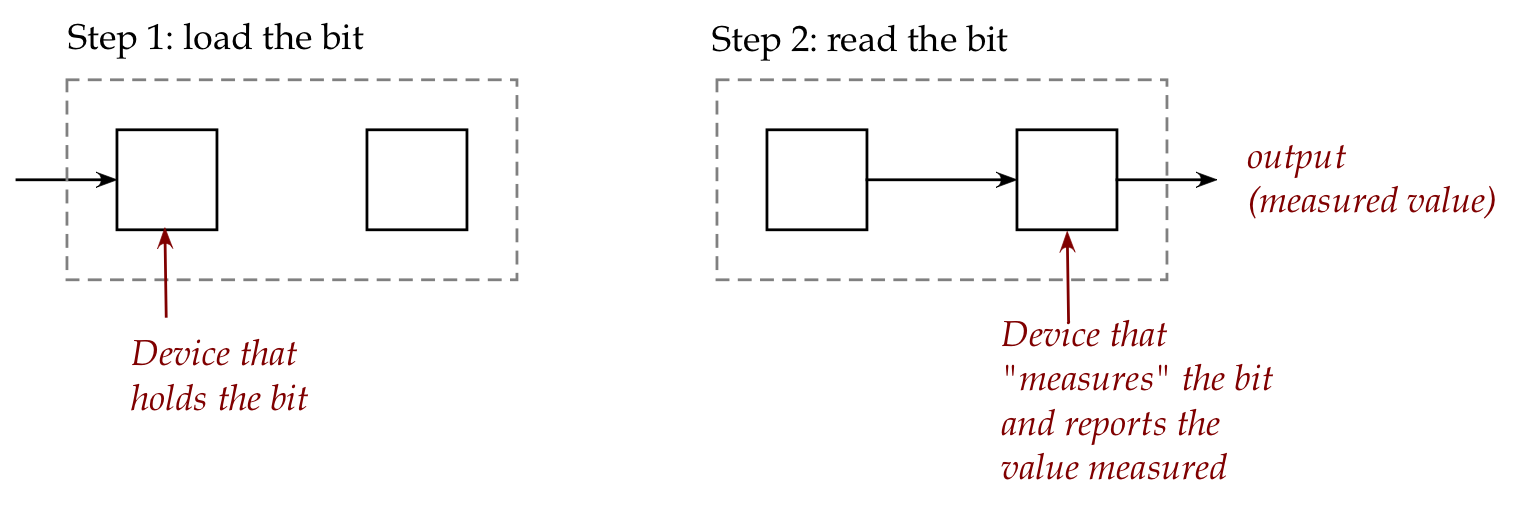
\includegraphics[width=4in]{notes/figs/n05/01bit1.png}
        \caption{Load and Read}
        \label{fig:01bit1}
    \end{figure}
    
    We'll now do an example and coalesce the two steps into a single diagram shown in Figure \ref{fig:02bit2}.

    \begin{figure}
        \centering
        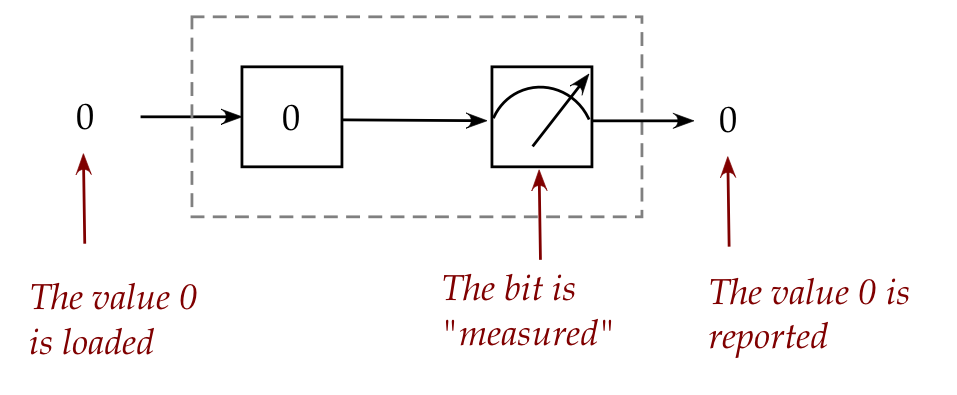
\includegraphics[width=4in]{notes/figs/n05/02bit2.png}
        \caption{Load Measure Report}
        \label{fig:02bit2}
    \end{figure}
    
    Let's point out: In practice the holding or storage device on the left is called a flip-flop. A flip-flop is a two-state device that can be thought of as: Low-voltage $\Rightarrow 0$, High-voltage $\Rightarrow 1$, The act of observing or measuring involves "spilling" of the electricity from the device to determine whether it's high or low ( 1 or 0 ). We're using an old-fashioned dial to label a measuring device. Notice that we've used the term measure instead of observe or read. This is the terminology used in quantum systems. Next, we're going to repeat this load-and-measure for several times with the following set up shown in Figure \ref{03bit3}.
    
    \begin{figure}
        \centering
        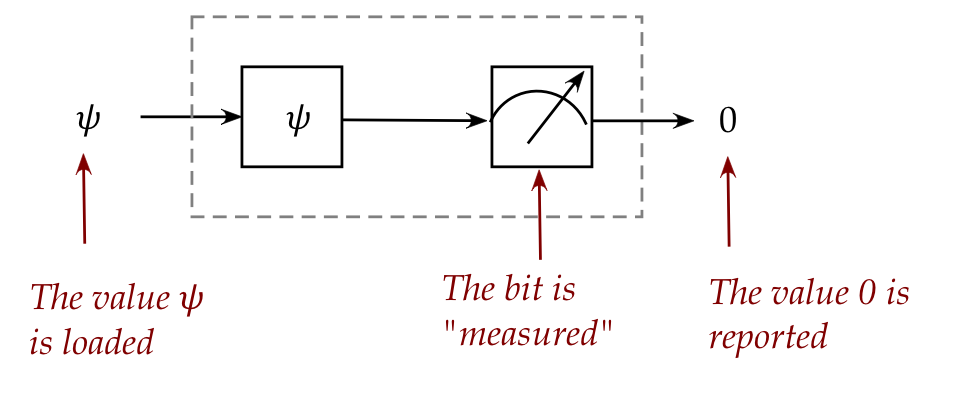
\includegraphics[width=4in]{notes/figs/n05/03bit3.png}
        \caption{load-and-measure for several times}
        \label{fig:03bit3}
    \end{figure}
    
    Someone, without telling us, loads the bit with a value unknown to us. We'll call this unknown value $\psi$. We then measure this value and report it. Let's say we observe 0. We now repeat the whole experiment (with loading) several times shown in Figure \ref{fig:04bit4}.
    
    \begin{figure}
        \centering
        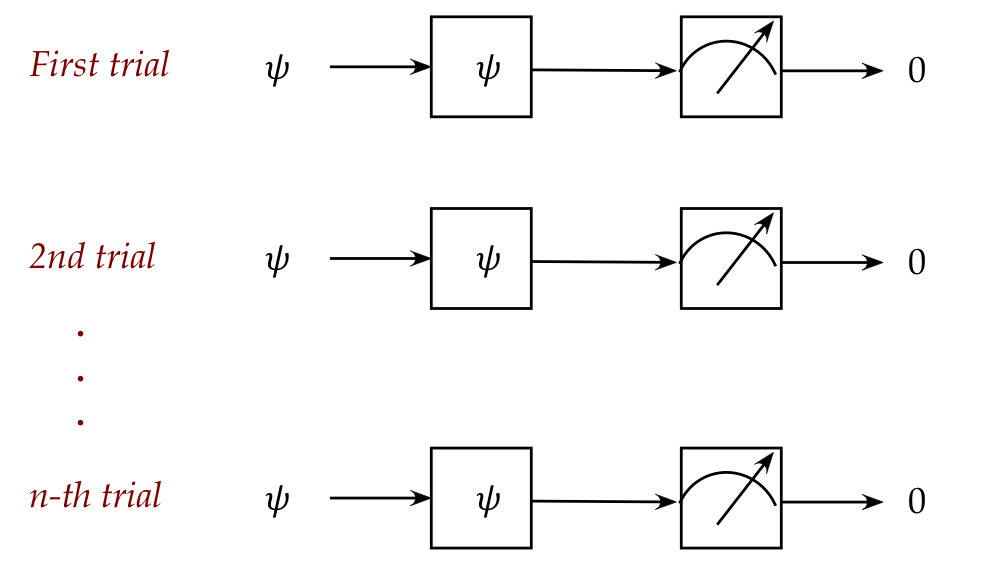
\includegraphics[width=4in]{notes/figs/n05/04bit4.png}
        \caption{experiment with loading several times}
        \label{fig:04bit4}
    \end{figure}
    
    We can assert three things with high confidence: 1. The unknown value $\psi$ is in fact 0. 2. Any number of repetitions will yield exactly the same result. 3. An alternative third-party measuring device will also yield exactly the same results (for this particular $\psi$ ). Surprisingly, none of these assertions can be made for a qubit. Let's now do the same experiment with a qubit: Qubit = Quantum bit Here's an example of some trials for a qubit shown in Figure \ref{fig:05qubit1}.
    
    \begin{figure}
        \centering
        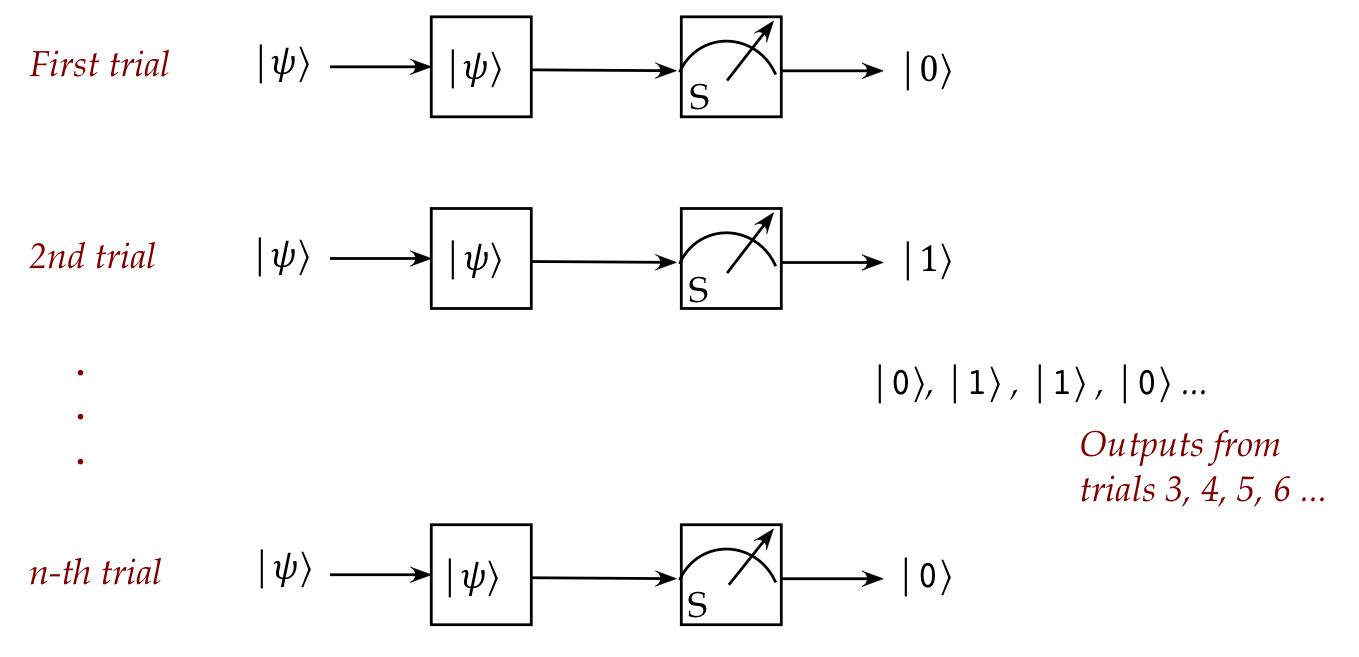
\includegraphics[width=4in]{notes/figs/n05/05qubit1.png}
        \caption{trials for a qubit}
        \label{fig:05qubit1}
    \end{figure}
    
    Note: We now cannot assert a definitive value for the unknown value $|\psi\rangle$. Multiple repetitions do not yield exactly the same value. In fact, statistical analysis over many trials shows that the pattern of output is completely random between $|0\rangle$ and $|1\rangle$. The measuring device performs an "S" measurement. (Whatever that means. We'll clarify later.) What if we used a different measuring device shown in Figure \ref{fig:06qubit2}.
    
    \begin{figure}
        \centering
        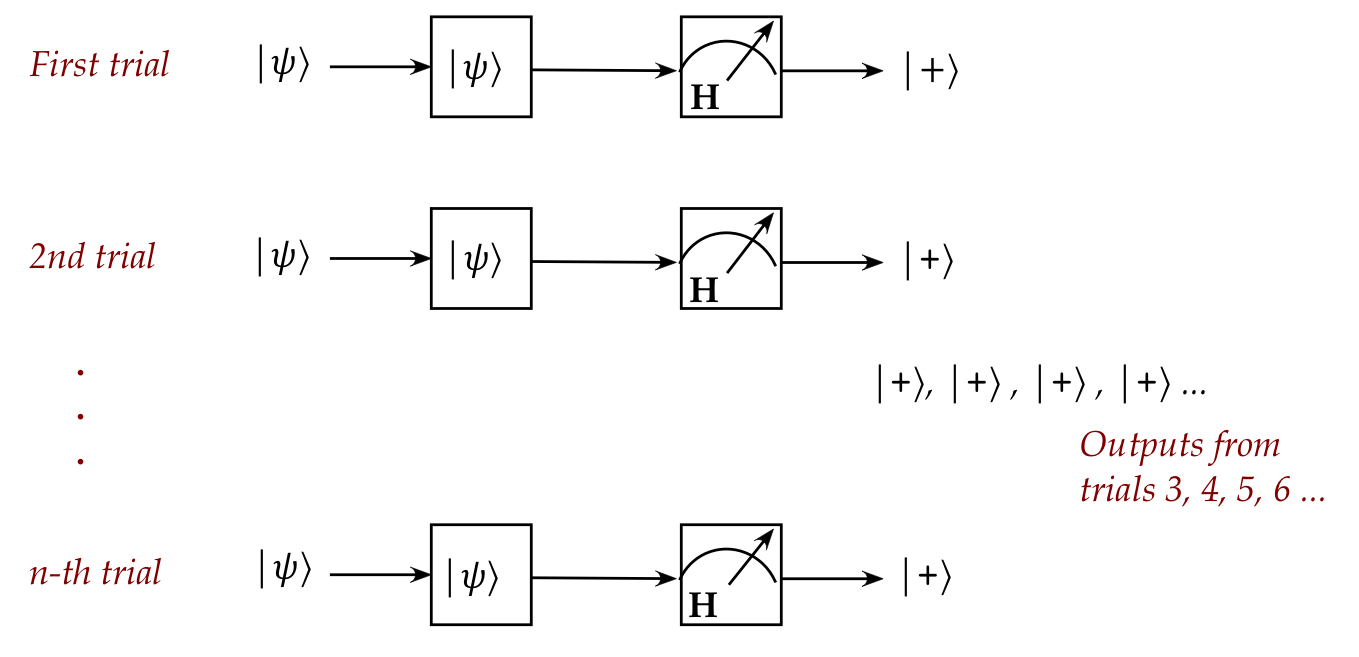
\includegraphics[width=4in]{notes/figs/n05/06qubit2.png}
        \caption{Different measuring device}
        \label{fig:06qubit2}
    \end{figure}
    
    Here, we have replaced an "S" device with an "H" measurement device. This time the output is entirely predictable! Does this remind you of anything from Module 1? Here's one Stern-Gerlach experiment shown in Figure \ref{fig:07sg1}.
    
    \begin{figure}
        \centering
        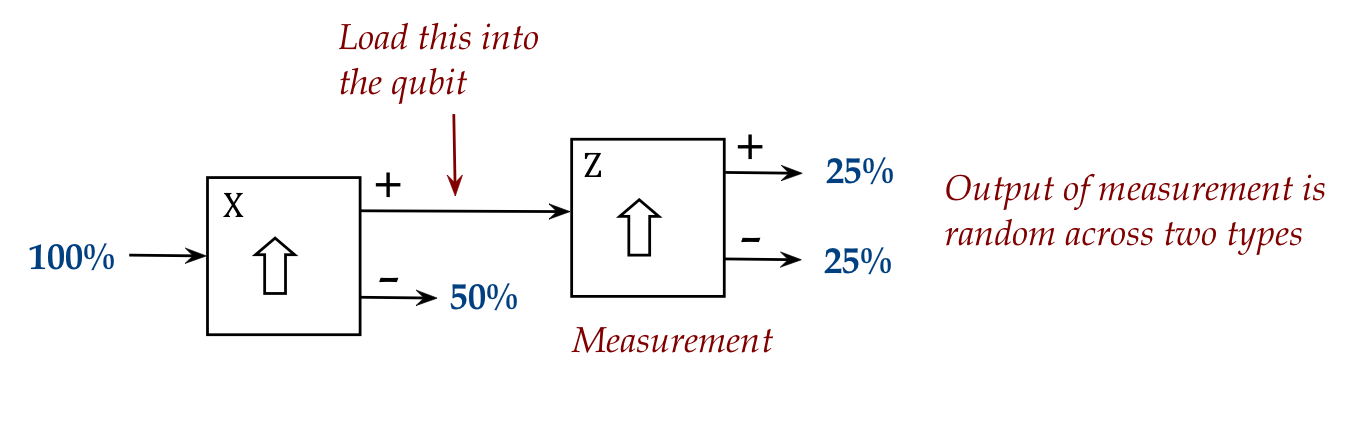
\includegraphics[width=4in]{notes/figs/n05/07sg1.png}
        \caption{Stern-Gerlach experiment}
        \label{fig:07sg1}
    \end{figure}
    
    The first state is X-aligned, the second is Z-aligned. Recall: the second-stage output is random between two types of output. A related SG experiment is shown in Figure \ref{fig:08sg2}.
    
    \begin{figure}
        \centering
        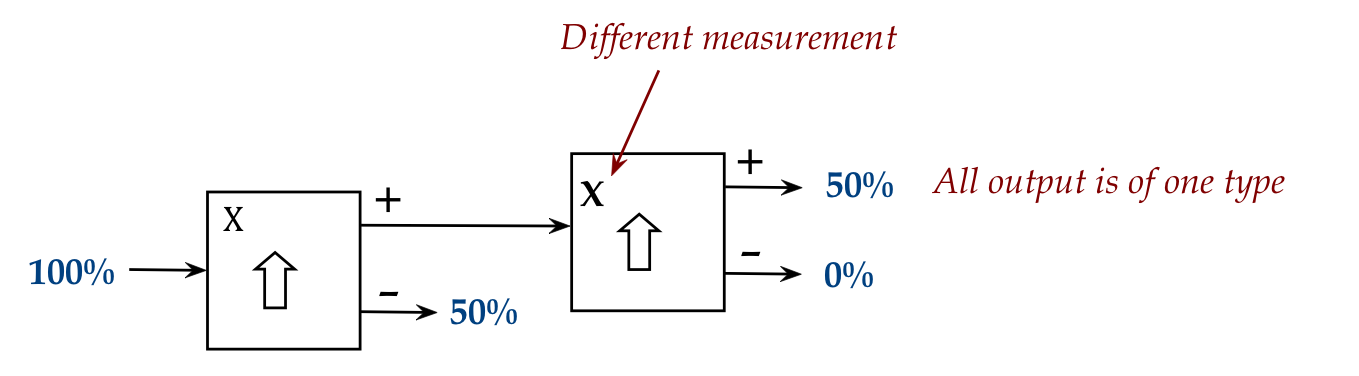
\includegraphics[width=4in]{notes/figs/n05/08sg2.png}
        \caption{Related Stern-Gerlach experiment}
        \label{fig:08sg2}
    \end{figure}
    
    Here, the output is consistently the same each time. In fact, a Stern-Gerlach apparatus is a qubit: There are many such two-level quantum systems that can serve as qubit technology. The SG apparatus is not at all practical. Other technologies are much more practical and successful. What's useful: the same theory works for all two-level systems (devices). So, what exactly is a qubit? Answer: A qubit is a device that holds a unit-length $2 D$ complex vector as its value. Consider for example, the complex vector
    
    $$
    |\psi\rangle=\left[\begin{array}{l}
    \alpha \\
    \beta
    \end{array}\right]
    $$
    
    Is $|\psi\rangle$ a qubit value? Yes! And it's a qubit value for any (unit-length) choice of the complex numbers $\alpha, \beta$. Example qubit values:
    
    $$
    |\psi\rangle=\left[\begin{array}{l}
    1 \\
    0
    \end{array}\right], \quad|\psi\rangle=\left[\begin{array}{l}
    0 \\
    1
    \end{array}\right], \quad|\psi\rangle=\left[\begin{array}{c}
    \frac{1}{\sqrt{2}} \\
    \frac{i}{\sqrt{2}}
    \end{array}\right]
    $$
    
    Note that a qubit vector can be expressed in any desired basis: Example: $|\psi\rangle=(\alpha, \beta)$ in the standard basis:
    
    $$
    |\psi\rangle=\left[\begin{array}{l}
    \alpha \\
    \beta
    \end{array}\right]=\alpha\left[\begin{array}{l}
    1 \\
    0
    \end{array}\right]+\beta\left[\begin{array}{l}
    0 \\
    1
    \end{array}\right]=\alpha|0\rangle+\beta|1\rangle
    $$
    
    Example: $|\psi\rangle=|0\rangle$ in the Hadamard basis:
    
    $$
    |0\rangle=\frac{1}{\sqrt{2}}|+\rangle+\frac{1}{\sqrt{2}}|-\rangle
    $$
    
    This is important, as we'll soon see. Terminology: The vector $|\psi\rangle$ that we've called the qubit's value is more often called the state of the qubit. $|\psi\rangle$ is also called the quantum state vector, and occasionally, the wavefunction. We can already see one implication: The set of possible values for a single qubit is (uncountably) infinite. Let's address the obvious question: do we impose the set of qubit values and then build hardware to support such qubits? No! This is what qubits are, and the theory follows from their natural behavior. All two-level quantum systems are modeled by 2D complex vectors This might be unsettling, but this is how nature is. There's more that's perplexing, as we'll see. We still need to address two issues: Where does the randomness come in? Why do we get different results with different types of measurements?
    
\subsection{Nature's indeterminism and the puzzle of measurement}

    Let's start with the measuring device: Think of a qubit measuring device as a 2D orthonormal basis: Example 1: Thus, for example, the basis
    
    $$
    \begin{aligned}
    &|0\rangle=\left[\begin{array}{l}
    1 \\
    0
    \end{array}\right] \\
    &|1\rangle=\left[\begin{array}{l}
    0 \\
    1
    \end{array}\right]
    \end{aligned}
    $$
    
    is one measuring device. Example 2: The basis
    
    $$
    \begin{aligned}
    |+\rangle &=\left[\begin{array}{l}
    \frac{1}{\sqrt{2}} \\
    \frac{1}{\sqrt{2}}
    \end{array}\right] \\
    |-\rangle=\left[\begin{array}{r}
    \frac{1}{\sqrt{2}} \\
    -\frac{1}{\sqrt{2}}
    \end{array}\right]
    \end{aligned}
    $$
    
    is another measuring device. In general, any orthonormal 2D basis
    
    $$
    \begin{aligned}
    |v\rangle &=a|0\rangle+b|1\rangle \\
    \left|v^{\perp}\right\rangle &=b^{*}|0\rangle-a^{*}|1\rangle
    \end{aligned}
    $$
    
    is a single qubit measuring device. Note: in $2 \mathrm{D},\left|v^{\perp}\right\rangle$ is the unique (unit-length) vector orthogonal to $(\backslash \mathrm{kt}\{\mathrm{v}\} \backslash)$. Now, any qubit state $|\psi\rangle$ can be expressed in terms of a measurement device's basis: For example, consider the basis $|0\rangle,|1\rangle$, and
   
    $$
    |\psi\rangle=\left[\begin{array}{l}
    \alpha \\
    \beta
    \end{array}\right]
    $$
    
    Then,
    
    $$
    |\psi\rangle=\alpha|0\rangle+\beta|1\rangle
    $$
    
    Another example: consider the basis $|+\rangle,|-\rangle$, and the vector $|\psi\rangle=|0\rangle$ :
    
    $$
    |\psi\rangle=\frac{1}{\sqrt{2}}|+\rangle+\frac{1}{\sqrt{2}}|-\rangle
    $$
    
    Now let's explain randomness and measurement outcome: The three aspects to a single measurement: 1. Every measurement of a qubit value is associated with a measurement basis. Example: $|0\rangle,|1\rangle$ 2. A particular measurement outcome will be a random selection from one of the basis vectors. Thus, either $|0\rangle$ or $|1\rangle$ 3. Which basis vector becomes the random outcome is based on these probabilities: Express the qubit's state in the measurement basis. Example: $|\psi\rangle=\langle 0 \mid \psi\rangle|0\rangle+\langle 1 \mid \psi\rangle|1\rangle$. This means each basis vector will have a coefficient in the expression: Example: $|\psi\rangle=\alpha|0\rangle+\beta|1\rangle$. The probability of seeing a particular basis vector is squared magnititude of the coefficient. Probability outcome is $|0\rangle=|\alpha|^{2}$. Probability outcome is $|1\rangle=|\beta|^{2}$. Example: Suppose we use the measurement basis $|0\rangle,|1\rangle$ and $|\psi\rangle=\alpha|0\rangle+\beta|1\rangle$ shown in Figure \ref{fig:09qubit3}.
    
    \begin{figure}
        \centering
        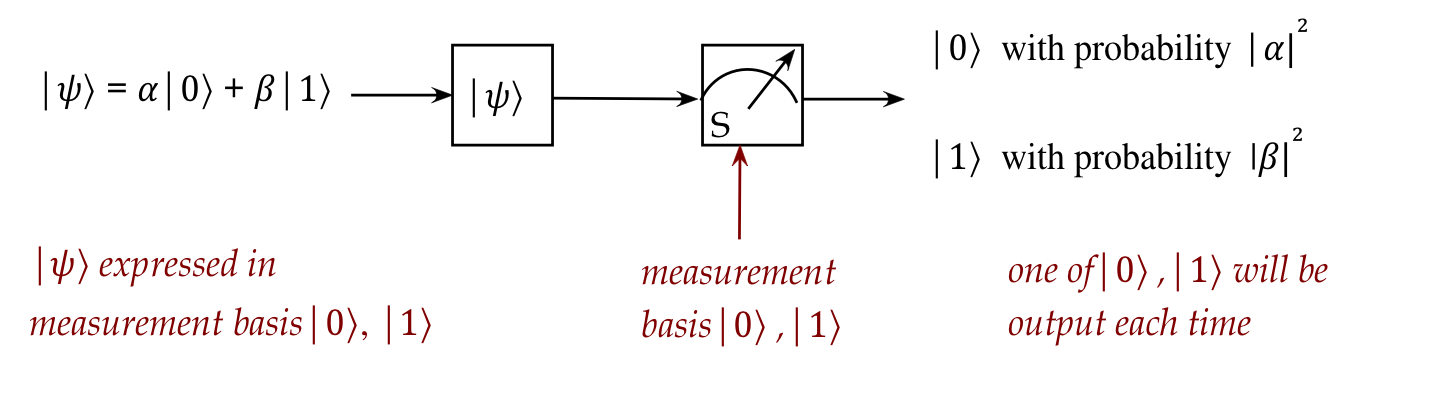
\includegraphics[width=4in]{notes/figs/n05/09qubit3.png}
        \caption{measurement basis $|0\rangle,|1\rangle$}
        \label{fig:09qubit3}
    \end{figure}
    
    Example: suppose we use the measurement basis $|+\rangle,|-\rangle$ and $|\psi\rangle=|0\rangle=\frac{1}{\sqrt{2}}|+\rangle+\frac{1}{\sqrt{2}}|-\rangle$ as shown in Figure \ref{fig:10qubit4}.
    
    \begin{figure}
        \centering
        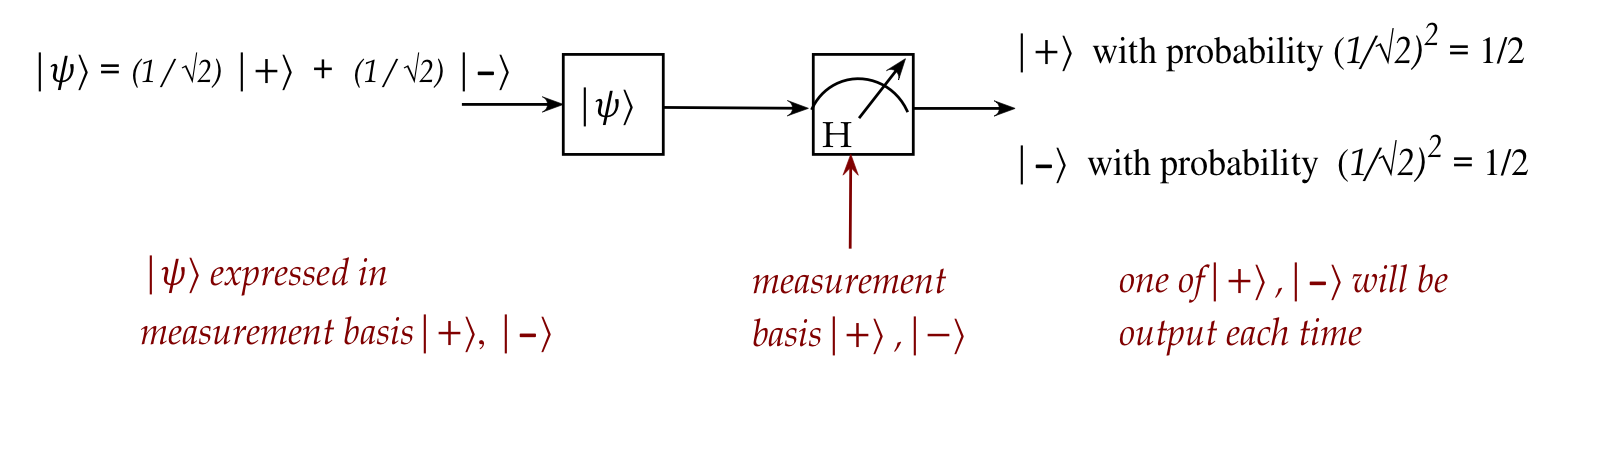
\includegraphics[width=4in]{notes/figs/n05/10qubit4.png}
        \caption{measurement basis $|+\rangle,|-\rangle$}
        \label{fig:10qubit4}
    \end{figure}
    
    Example: Suppose we use the measurement basis $|0\rangle,|1\rangle$ and $\psi=|0\rangle$ as shown in Figure \ref{fig:11qubit5}.
    
    \begin{figure}
        \centering
        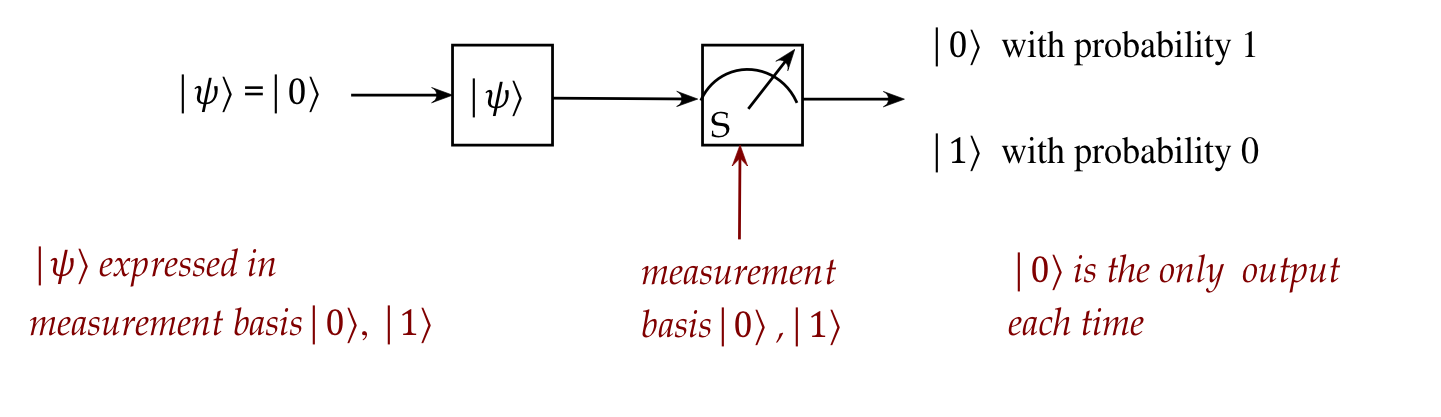
\includegraphics[width=4in]{notes/figs/n05/11qubit5.png}
        \caption{measurement basis $|0\rangle,|1\rangle$ }
        \label{fig:11qubit5}
    \end{figure}
    
    There is a more general way of describing measurement, called projective measurement, that we'll see later. Let's say a bit more about measurement: First, why is the output random? One might wonder: are measurement devices deliberately constructed to perform random selection? And if so, why would anyone want to do that? The answer to the first: No! This is just how nature $i$ s. The only time the measurement is not random is when the outcome probability for one of the basis vectors is $1 .$ $\triangleright$ The case when the input is, in fact, that basis vector. In general, any measurement of any quantum state (in any quantum device) is going to involve random output. That is, one cannot construct a measurement device that avoids the randomness for all (even most) states. Why do we bother with measurement when the outcome is uncertain? Why not just observe the qubit value? This is another unsettling issue: the only way to know a qubit's state is to measure it. To summarize so far: To examine a qubit's state, one must measure. A measurement outcome is random, and is one of the measurement-basis vectors. There's yet another issue: Measurement changes the qubit's state into one of the basis vectors. That is, it is not possible to measure a qubit and leave the qubit in its original state. (We'll say more about this in the next section.) Another piece of the puzzle shown in Figure \ref{fig:12qubit5b}.
    
    \begin{figure}
        \centering
        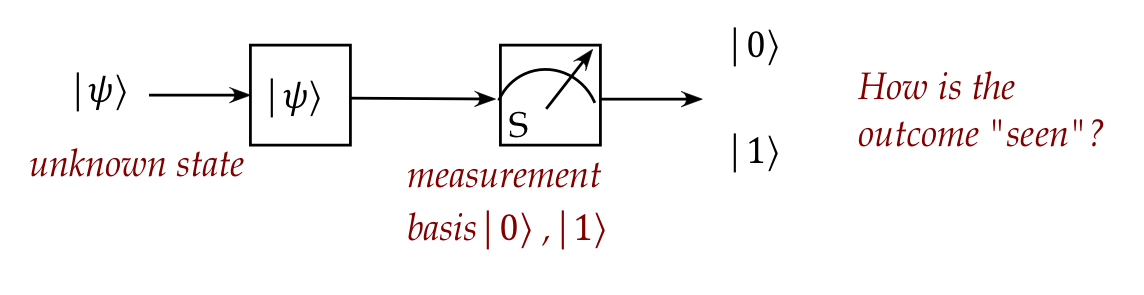
\includegraphics[width=4in]{notes/figs/n05/12qubit5b.png}
        \caption{unknown state}
        \label{fig:12qubit5b}
    \end{figure}
    
    We have said that a state cannot be observed, only measured. How then do we know which measurement outcome state occurred? Isn't that a form of observation? A measurement is accompanied by a physical value that can be observed, such as energy (frequency) shown in Figure \ref{fig:13qubit5c}.
    
    \begin{figure}
        \centering
        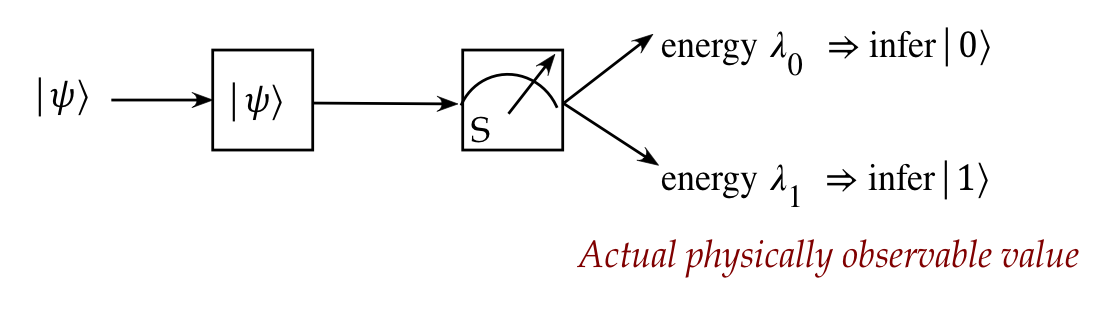
\includegraphics[width=4in]{notes/figs/n05/13qubit5c.png}
        \caption{Physically observable state}
        \label{fig:13qubit5c}
    \end{figure}
    
    Every unique outcome has a unique accompanying physical value: If this sounds suspiciously like "different eigenvectors have different eigenvalues". That's because it is the case! Actual measurement hardware detects the value of the accompanying physical value or signal.

\subsection{Stationary vs flying qubits}

    We will distinguish between are two types of hardware configurations: stationary and flying qubits. Both are identical in terms of theory, and so we will (as do all books) use only the latter because it's more convenient to draw. Think of a flying qubit as an atom or photon in motion: Consider a flying qubit $|\psi\rangle=\alpha|0\rangle+\beta|1\rangle$ entering a standard-basis measuring device. Suppose measurement resulted in $|0\rangle$ as shown in Figure \ref{fig:14qubit8}.
    
    \begin{figure}
        \centering
        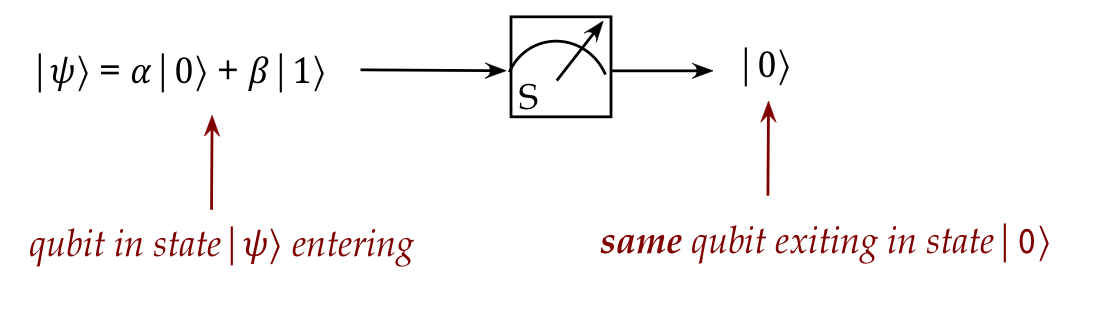
\includegraphics[width=4in]{notes/figs/n05/14qubit8.png}
        \caption{measurement resulted in $|0\rangle$}
        \label{fig:14qubit8}
    \end{figure}
    
    A qubit enters from the left (in this picture) in the $\alpha|0\rangle+\beta|1\rangle$ state. After measurement, it's new state is $|0\rangle$. That is, there's only one qubit in play here. The changed qubit can now be directed towards other devices, perhaps to a measurement in another basis. Think of a stationary qubit as the state of an atom's outermost electron: For example, here are three qubits in three different states shown in Figure \ref{fig:15qubit6}.
    
    \begin{figure}
        \centering
        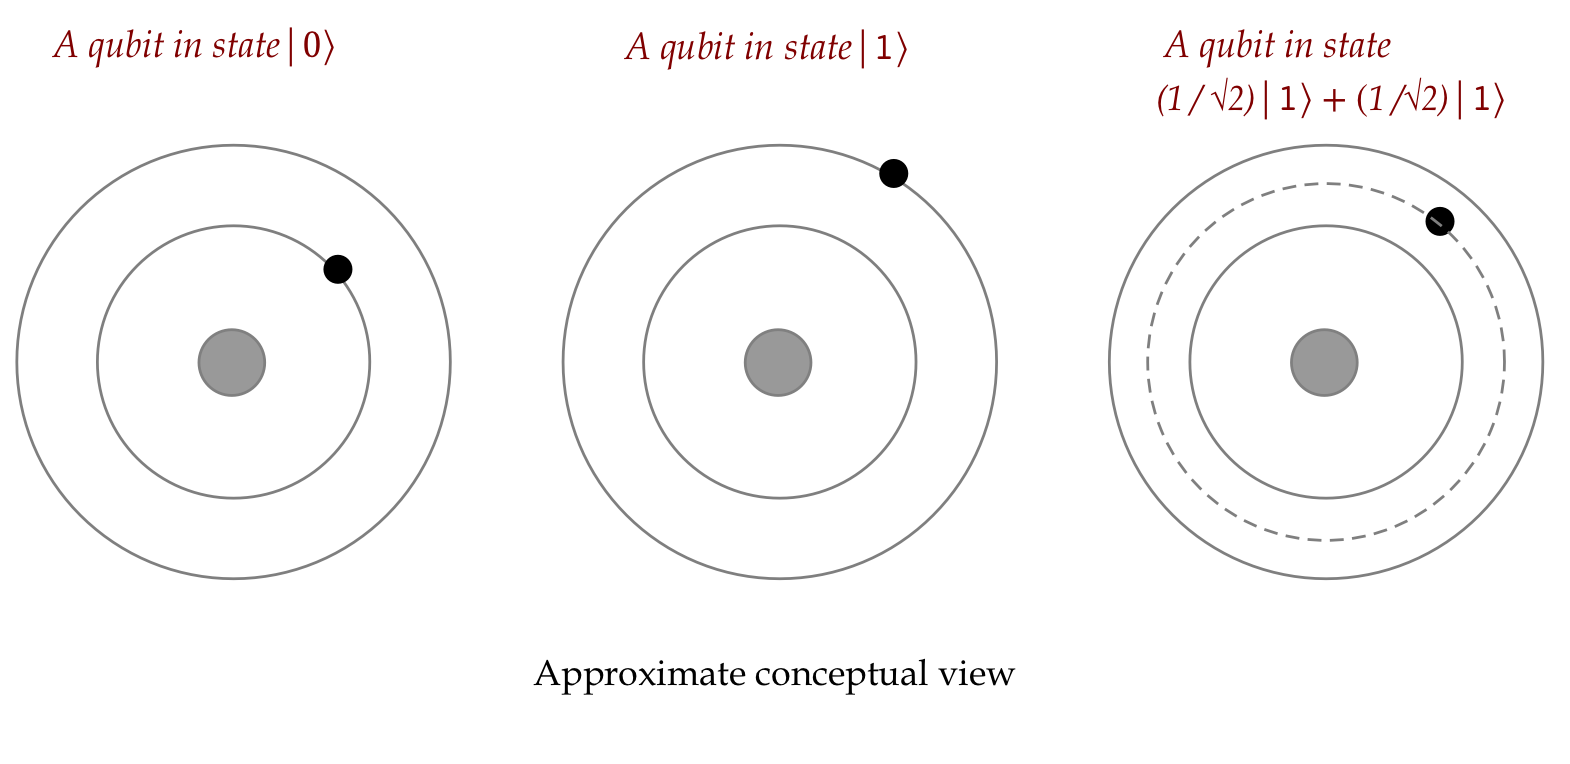
\includegraphics[width=4in]{notes/figs/n05/15qubit6.png}
        \caption{Three qubits in three different states}
        \label{fig:15qubit6}
    \end{figure}
    
    Here: Here, $|0\rangle$ is typically the lowest energy or ground state of the electron. $|1\rangle$ is the excited state. The state $\frac{1}{\sqrt{2}}|0\rangle+\frac{1}{\sqrt{2}}|1\rangle$ is depicted above, on the right. Note: The above depiction is only an approximation for a simplified high-level conceptual view. The actual location of an electron, and this "planetary motion" view is actually not correct. It's more accurate to say the electron is in a quantum state, to which various measurements can be made, including location, momentum, and other properties. How does measurement work for a stationary qubit? Reference Figure \ref{fig:16qubit7}.
    
    \begin{figure}
        \centering
        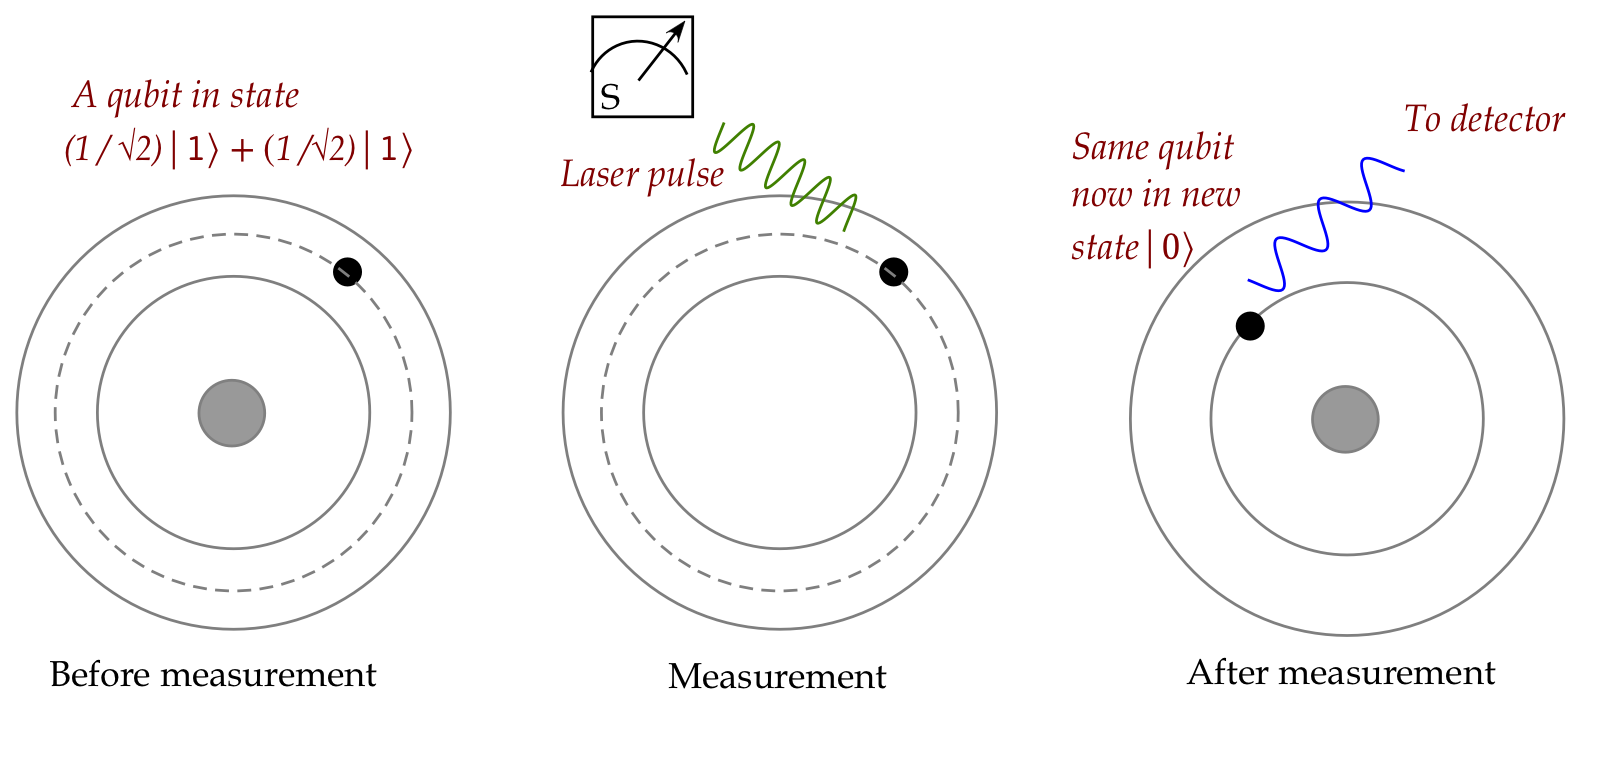
\includegraphics[width=4in]{notes/figs/n05/16qubit7.png}
        \caption{measurement for stationary qubit}
        \label{fig:16qubit7}
    \end{figure}
    
    Here, the measurement device is brought to the qubit and activated. This changes the state of the qubit. There is some additional output that tells a detector whether the post-measurement state is $|0\rangle$ or $|1\rangle$. The measurement device is then deactivated. Thus, using our conceptual boxes, we should really have drawn something like Figure \ref{fig:17qubit8}.
    
    \begin{figure}
        \centering
        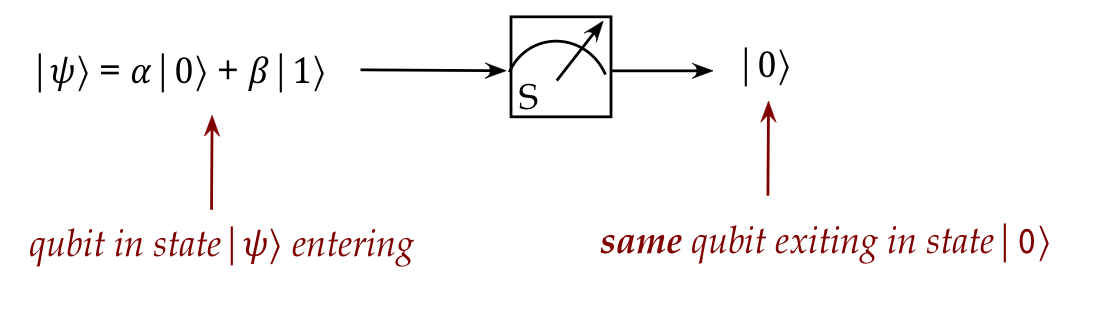
\includegraphics[width=4in]{notes/figs/n05/17qubit8.png}
        \caption{qubit state entering and exiting}
        \label{fig:17qubit8}
    \end{figure}
    
    The stationary kind of qubit is the more common technology, and the one considered the most likely for quantum computing. The convention in drawing: The theory is exactly the same for both types of qubit configurations. The convention in books is to use the flying qubit diagram shown in Figure \ref{fig:18qubit10}.
    
    \begin{figure}
        \centering
        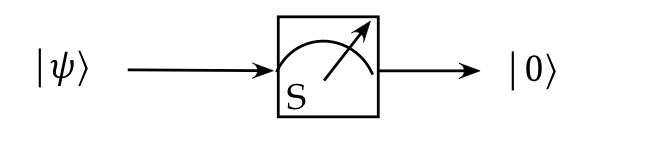
\includegraphics[width=4in]{notes/figs/n05/18qubit10.png}
        \caption{flying qubit}
        \label{fig:18qubit10}
    \end{figure}
    
    Measurement and initialization: Suppose we want to initalize a qubit into state $|0\rangle$. At the start, suppose a qubit is in an unknown state $|\psi\rangle$. We perform a measurement in the $|0\rangle,|1\rangle$ basis. If this results in state $|0\rangle$, we're done. We know that the state is now $|0\rangle$. If not, we can change the state (next section) and apply measurement again, repeating this whole process until a measurement outcome is $|0\rangle$.

\subsection{What can you do with a qubit?}

    If all we could do is measure, we would not get far with quantum computing. Luckily, nature lets us modify a qubit's state without measurement. However, there's one limitation: The only modification allowed is a unitary operation. Let's look at an example: Consider the unitary operator
    
    $$
    \left[\begin{array}{ll}
    0 & 1 \\
    1 & 0
    \end{array}\right]
    $$
    
    Let's ask: what would we get if we applied this to a qubit in state $|0\rangle$ ?
    
    $$
    X|0\rangle=\left[\begin{array}{ll}
    0 & 1 \\
    1 & 0
    \end{array}\right]\left[\begin{array}{l}
    1 \\
    0
    \end{array}\right]=\left[\begin{array}{l}
    0 \\
    1
    \end{array}\right]=|1\rangle
    $$
    
    We will diagram this as Figure \ref{fig:19gate4}.
    
    \begin{figure}
        \centering
        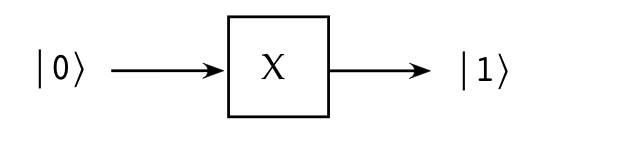
\includegraphics[width=4in]{notes/figs/n05/19gate1.png}
        \caption{}
        \label{fig:19gate4}
    \end{figure}
    
    Note that
    
    $$
    X|1\rangle=\left[\begin{array}{ll}
    0 & 1 \\
    1 & 0
    \end{array}\right]\left[\begin{array}{l}
    0 \\
    1
    \end{array}\right]=\left[\begin{array}{l}
    1 \\
    0
    \end{array}\right]=|0\rangle
    $$
    
    which we can depict as Figure \ref{fig:20polarizer1}.
    
    \begin{figure}
        \centering
        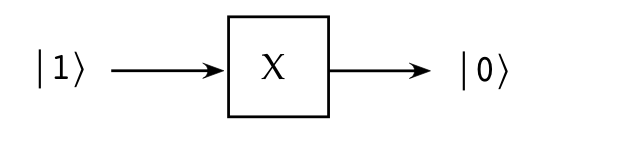
\includegraphics[width=4in]{notes/figs/n05/20gate2.png}
        \caption{}
        \label{fig:20polarizer1}
    \end{figure}
    
    Observe that applying $X$ twice results in
    
    $$
    X X=\left[\begin{array}{ll}
    0 & 1 \\
    1 & 0
    \end{array}\right]\left[\begin{array}{ll}
    0 & 1 \\
    1 & 0
    \end{array}\right]=\left[\begin{array}{ll}
    1 & 0 \\
    0 & 1
    \end{array}\right]
    $$

    That is, the original state is returned.
    
    Another example: Consider the Hadamard matrix
    
    $$
    H=\left[\begin{array}{cc}
    \frac{1}{\sqrt{2}} & \frac{1}{\sqrt{2}} \\
    \frac{1}{\sqrt{2}} & -\frac{1}{\sqrt{2}}
    \end{array}\right]
    $$
    
    This is unitary as can be seen:
    
    $$
    H^{\dagger} H=\left[\begin{array}{cc}
    \frac{1}{\sqrt{2}} & \frac{1}{\sqrt{2}} \\
    \frac{1}{\sqrt{2}} & -\frac{1}{\sqrt{2}}
    \end{array}\right]\left[\begin{array}{cc}
    \frac{1}{\sqrt{2}} & \frac{1}{\sqrt{2}} \\
    \frac{1}{\sqrt{2}} & -\frac{1}{\sqrt{2}}
    \end{array}\right]=I
    $$
    
    Thus, it can be used to modify a qubit's state. An aside: We've seen the H matrix in many roles. For example, it was a change-of-basis matrix. And because it's Hermitian, it served as an example then. The Hadamard matrix is one of the most important tools in quantum computing. Now let's see what it does to $|0\rangle,|1\rangle$ :
    
    $$
    \begin{aligned}
    &H|0\rangle=\left[\begin{array}{cc}
    \frac{1}{\sqrt{2}} & \frac{1}{\sqrt{2}} \\
    \frac{1}{\sqrt{2}} & -\frac{1}{\sqrt{2}}
    \end{array}\right]\left[\begin{array}{l}
    1 \\
    0
    \end{array}\right]=\left[\begin{array}{c}
    \frac{1}{\sqrt{2}} \\
    \frac{1}{\sqrt{2}}
    \end{array}\right]=|+\rangle \\
    &H|1\rangle=\left[\begin{array}{cc}
    \frac{1}{\sqrt{2}} & \frac{1}{\sqrt{2}} \\
    \frac{1}{\sqrt{2}} & -\frac{1}{\sqrt{2}}
    \end{array}\right]\left[\begin{array}{l}
    0 \\
    1
    \end{array}\right]=\left[\begin{array}{r}
    \frac{1}{\sqrt{2}} \\
    -\frac{1}{\sqrt{2}}
    \end{array}\right]=|-\rangle
    \end{aligned}
    $$
    
    Thus, the H operator transforms the state $|0\rangle$ into the state $|+\rangle$; transforms the state $|1\rangle$ into the state $|-\rangle$; What does it do to the general standard-basis vector $|\psi\rangle=\alpha|0\rangle+\beta|1\rangle$ ?
    
    $$
    H|\psi\rangle=\frac{\alpha+\beta}{\sqrt{2}}|0\rangle+\frac{\alpha-\beta}{\sqrt{2}}|1\rangle
    $$
    
    Now let's build our first circuit in Figure \ref{fig:21polarizer1b}.
    
    \begin{figure}
        \centering
        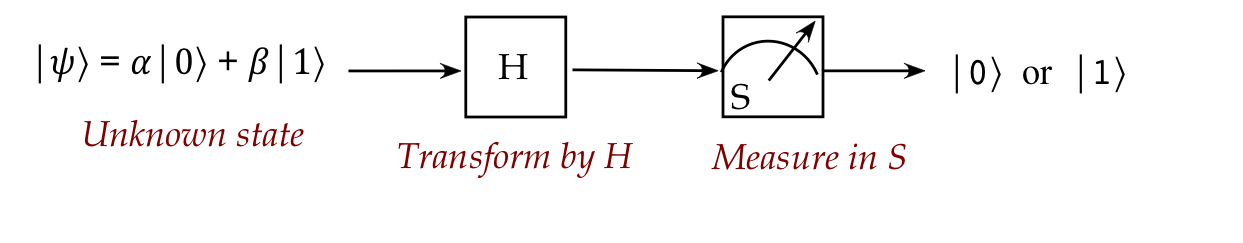
\includegraphics[width=4in]{notes/figs/n05/21gate3.png}
        \caption{Unknown state, transform, measure}
        \label{fig:21polarizer1b}
    \end{figure}
    
    We have an unknown state $|\psi\rangle=\alpha|0\rangle+\beta|1\rangle$ entering from the left. Applying the $\mathrm{H}$ transform results in
    
    $$
    H|\psi\rangle=\frac{\alpha+\beta}{\sqrt{2}}|0\rangle+\frac{\alpha-\beta}{\sqrt{2}}|1\rangle
    $$
    
    Measuring in the standard basis yields $|0\rangle$ with probability $\left|\frac{\alpha+\beta}{\sqrt{2}}\right|^{2}$, $|1\rangle$ with probability $\left|\frac{\alpha-\beta}{\sqrt{2}}\right|^{2}$. Suppose we perform this experiment several times and obtain $|0\rangle$ much more often than $|0\rangle$. This means the probability of obtaining $|0\rangle$ is much higher than the probability of getting $|0\rangle$. That is,
    
    $$
    \begin{aligned}
    &\left|\frac{\alpha+\beta}{\sqrt{2}}\right|^{2} \approx 1 \\
    &\left|\frac{\alpha-\beta}{\sqrt{2}}\right|^{2} \approx 0
    \end{aligned}
    $$
    
    From which we conclude $\alpha \approx \beta$. Thus, we've learned something about the unknown state through a simple transformation. Of course, we could measure the unknown state repeatedly and estimate in that manner too, but if we skew the probabilities as above, we can arrive at the same result sooner.
    Another example: Consider the strangely-named matrix
    
    $$
    \sqrt{X}=\left[\begin{array}{cc}
    \frac{1+i}{2} & \frac{1-i}{2} \\
    \frac{1-i}{2} & \frac{1+i}{2}
    \end{array}\right]
    $$
    
    Is it unitary?
    
    $$
    (\sqrt{X})^{\dagger}=\left[\begin{array}{cc}
    \frac{1-i}{2} & \frac{1+i}{2} \\
    \frac{1+i}{2} & \frac{1-i}{2}
    \end{array}\right]
    $$
    
    Then it's easy to calculate
    
    $$
    (\sqrt{X})^{\dagger} \sqrt{X}=I
    $$
    
    Observe that
    
    $$
    \sqrt{X} \sqrt{X}=\left[\begin{array}{cc}
    \frac{1+i}{2} & \frac{1-i}{2} \\
    \frac{1-i}{2} & \frac{1+i}{2}
    \end{array}\right]\left[\begin{array}{cc}
    \frac{1+i}{2} & \frac{1-i}{2} \\
    \frac{1-i}{2} & \frac{1+i}{2}
    \end{array}\right]=\left[\begin{array}{ll}
    0 & 1 \\
    1 & 0
    \end{array}\right]=X
    $$
    
    Thus, the effect of applying $\sqrt{X}$ twice is the same as applying $X$. While $X$ has a natural classical analog, the NOT Boolean gate, $\sqrt{X}$ has no classical analog. Some terminology: A unitary operator is called a quantum gate, or just gate. Superposition: A vector such as $\frac{1}{\sqrt{2}}|0\rangle+\frac{1}{\sqrt{2}}|1\rangle$ or $\alpha|0\rangle+\beta|1\rangle$ that is a linear combination of basis vectors is sometimes called a superposition. About superpositions: Any superposition requires specifying the basis used in the linear combination. A superposition is not a simultaneous occurrence of the basis vectors involved. It's just a vector that happens to be expressible as a linear combination of basis vectors. Clearly, a particular vector can be a superposition in one basis (e.g., $\left.|+\rangle=\frac{1}{\sqrt{2}}|0\rangle+\frac{1}{\sqrt{2}}|1\rangle\right)$ but not so in another basis (e.g, $|+\rangle$ in the $|+\rangle,|-\rangle$ basis). Figure \ref{fig:22gate4}.
    
    \begin{figure}
        \centering
        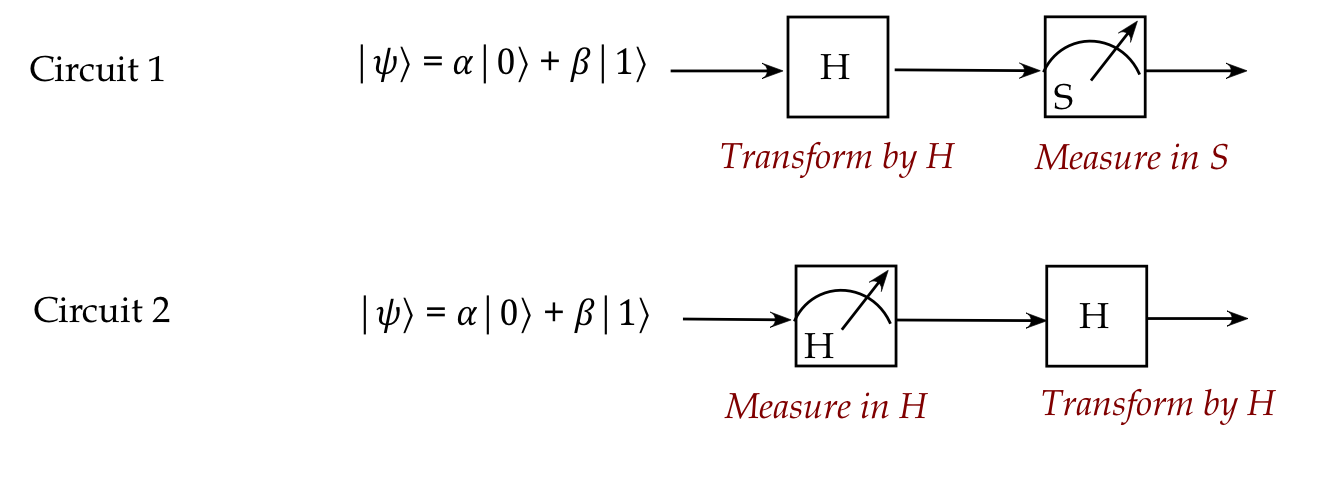
\includegraphics[width=4in]{notes/figs/n05/22gate4.png}
        \caption{Transform Measure, Measure Transform}
        \label{fig:22gate4}
    \end{figure}
    
\subsection{The promise and challenge of quantum computing viewed through a qubit}

    What we've seen so far gives us a hint of the promise and challenge in quantum computing. First, the promise: Compared to a regular bit, a qubit can be in one of an infinite number of states. A unitary operator can be applied to any qubit, not just the two standard-basis states $|0\rangle,|1\rangle$. It's natural to equate $|0\rangle,|1\rangle$ with regular bits 0 and $1 .$ We will later see how regular logic circuits can be converted to quantum equivalents, showing that a quantum circuit can do what a logic circuit can do. But quantum states are many more! Consider the state
    
    $$
    |+\rangle=\frac{1}{\sqrt{2}}|0\rangle+\frac{1}{\sqrt{2}}|1\rangle
    $$
    
    This is a linear combination of the two states $|0\rangle,|1\rangle$ : It is incorrect to think of this as a "mixture" of the two states $|0\rangle,|1\rangle$. $|+\rangle$ is a state, period. It can be expressed as a linear combination of all kinds of basis vectors. We will later see that it's possible to create a 2-qubit state like
    
    $$
    \frac{1}{2}(|00\rangle+|01\rangle+|10\rangle+|11\rangle)
    $$
    
    That is, a combination of all four 2-qubit basis states. In fact, we'll see that with n qubits, one can create a state that combines all $2^{n}$ basis states! This suggests that we can compute simultaneously with all of them. In fact, this is often the starting point for many quantum algorithms. There is a multi-qubit property called entanglement that's both mystifying and powerful, which we will exploit. In combination, all these properties show that quantum computers can: perform some computations that no classical computer can; perform some computations provably faster than a classical computer (so-called quantum supremacy). But ... there are many challenges in exploiting this power: Measurement has probabilistic outcomes: This may mean repeating a computation until one has a result with high probability. Measurement destroys quantum state, replacing it with one of the measurement basis vectors: This means one typically uses measurement only after a sequence of unitary operations. Although, as we will see later, unitary operations can simulate any classical logic circuit, there are added gates needed, which impacts efficiency. These are just the theoretical "in principle" challenges. The hardware challenges are even more significant: Quantum states don't last long and thus unitary operations must be performed quickly. The slightest bit of noise can derail any computation. This is called decoherence. It's difficult to work with multiple qubits. Currently, hardware needed for cooling is expensive. Nonetheless, as of 2022, leading vendors claim to have demonstrated computations on over a dozen error-corrected qubits.

\subsection{Revisiting the light polarization experiment}

    Recall the phenomenon of polarization shown in Figure \ref{fig:23polarizer1}.
    
    \begin{figure}
        \centering
        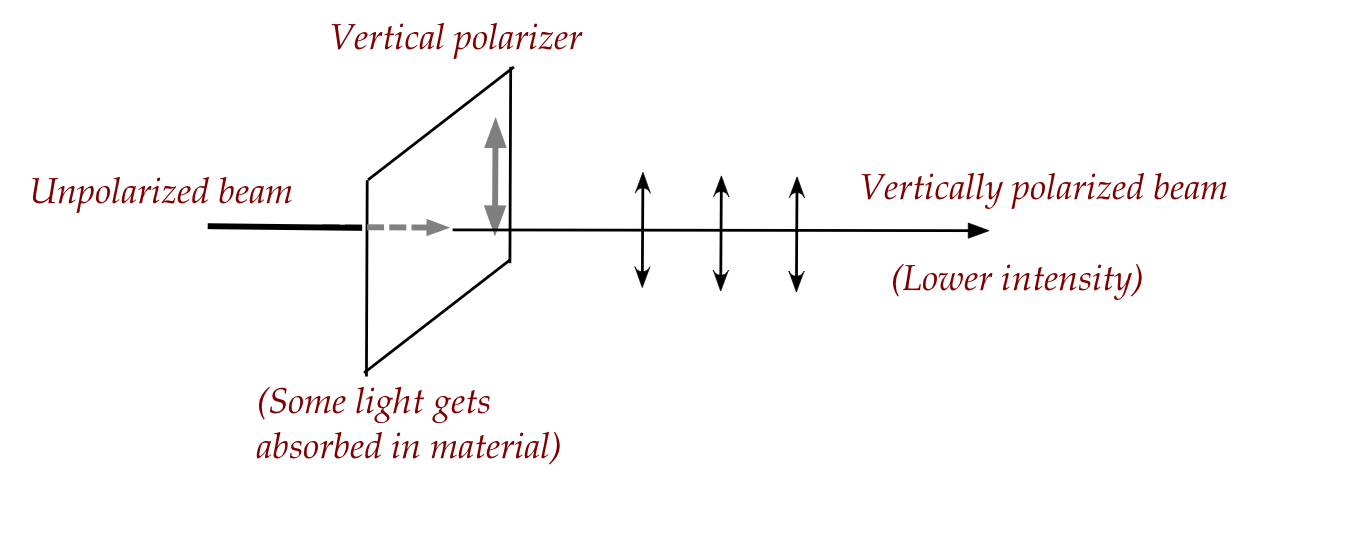
\includegraphics[width=4in]{notes/figs/n05/23polarizer1.png}
        \caption{Unpolarized beam, Polarized beam}
        \label{fig:23polarizer1}
    \end{figure}
    
    The same experiment with single photons in Figure \ref{fig:24polarizer1b}.
    
    \begin{figure}
        \centering
        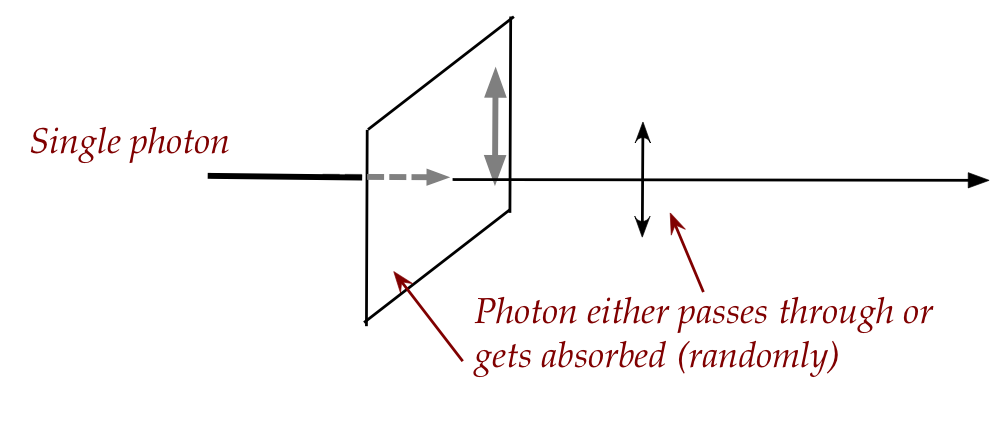
\includegraphics[width=4in]{notes/figs/n05/24polarizer1b.png}
        \caption{Single Photon}
        \label{fig:24polarizer1b}
    \end{figure}
    
    Now consider the first of two experiments in Figure \ref{fig:25polarizer2}.
    
    \begin{figure}
        \centering
        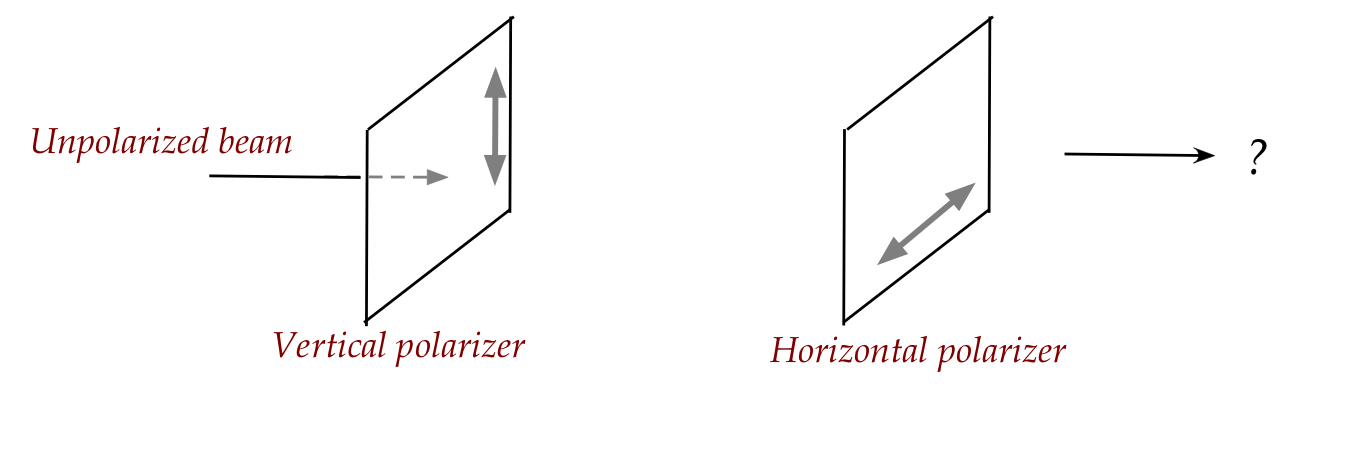
\includegraphics[width=4in]{notes/figs/n05/25polarizer2.png}
        \caption{Vertical polarizer, Horizontal polarizer}
        \label{fig:25polarizer2}
    \end{figure} 
    
    In this scenario: Careful experimentation shows that: no light emerges from the second polarizer. The same result obtains when sending a single photon at a time. For single photons: The photon either gets absorbed or passes through the first polarizer. A photon that passes the first is always absorbed by the second polarizer. Now consider the second scenario in Figure \ref{fig:26polarizer3}.
    
    \begin{figure}
        \centering
        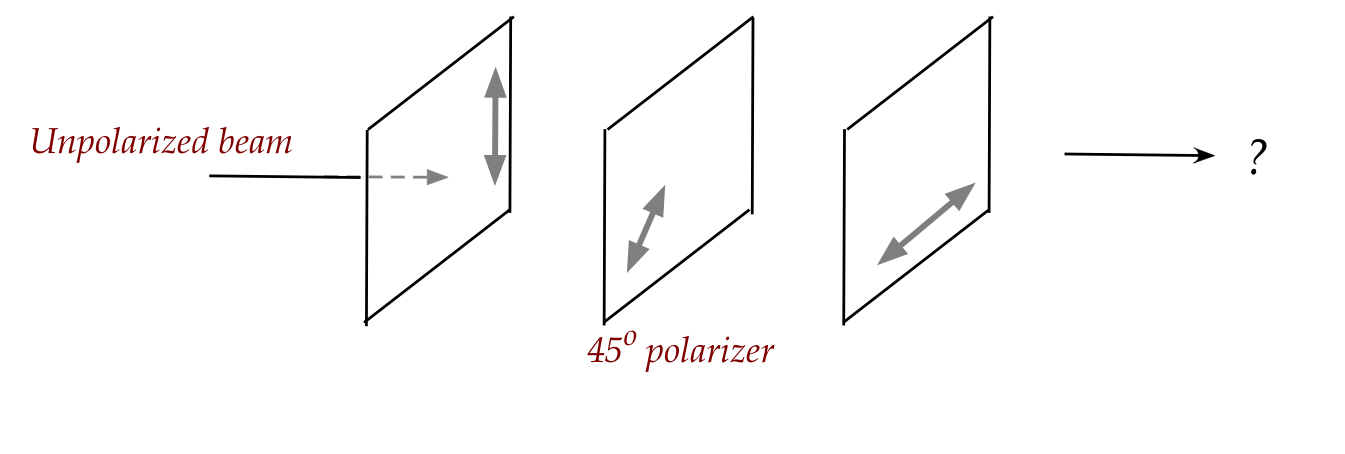
\includegraphics[width=4in]{notes/figs/n05/26polarizer3.png}
        \caption{45 degree polarizer}
        \label{fig:26polarizer3}
    \end{figure} 
    
    In this case in Figure \ref{fig:27polarizer4}.

    \begin{figure}
        \centering
        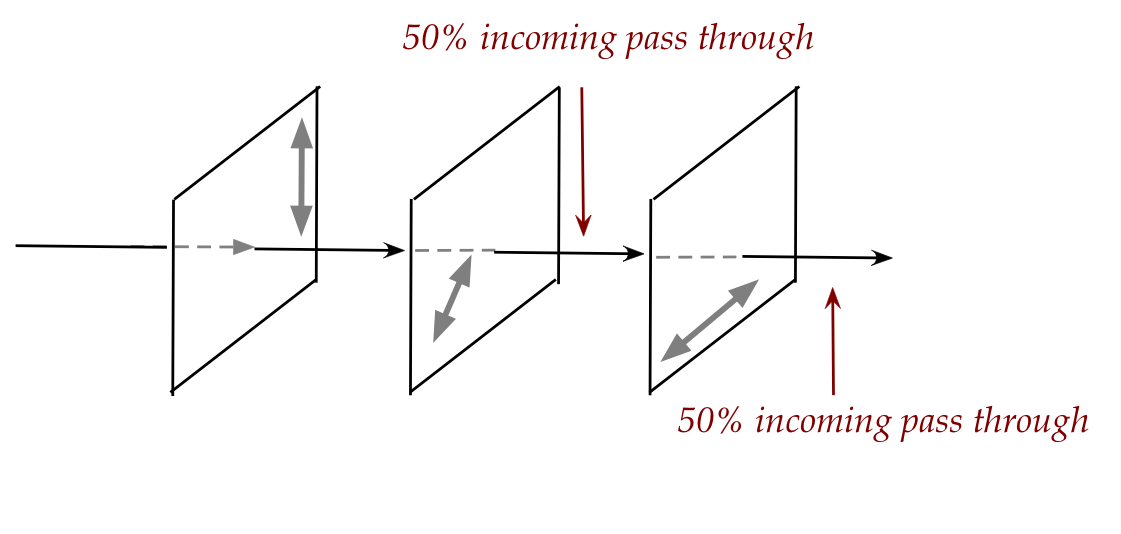
\includegraphics[width=4in]{notes/figs/n05/27polarizer4.png}
        \caption{50 percentage incoming pass through}
        \label{fig:27polarizer4}
    \end{figure} 
    
    Photons are randomly either absorbed or pass through the first polarizer. Here's the key observation: $50 \%$ of the photons that reach the middle polarizer pass through. Of the photons that reach the third, $50 \%$ pass through. While a classical explanation can be constructed for beams of light, no classical reasoning explains the single-photon experiments. Now let's provide a quantum explanation shown in Figure \ref{fig:28polarizer5}.
    
    \begin{figure}
        \centering
        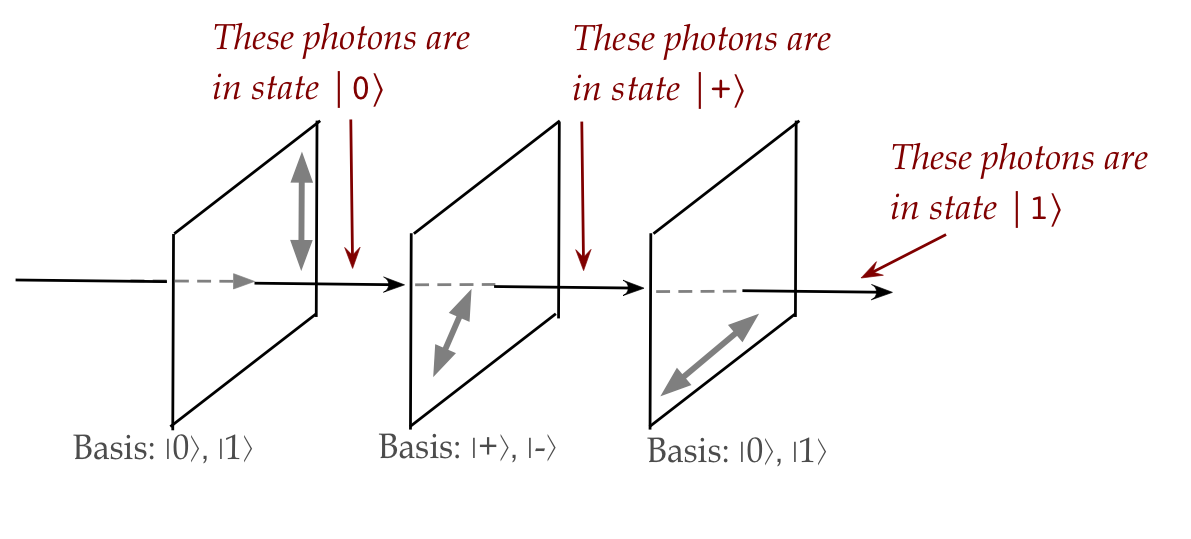
\includegraphics[width=4in]{notes/figs/n05/28polarizer5.png}
        \caption{photon states}
        \label{fig:28polarizer5}
    \end{figure}
    
    Each polarizer is a measuring device. The bases used by the first and third are: The first polarizer uses: $|0\rangle=$ pass through, vertically polarized $|1\rangle=$ absorb. The third polarizer uses: $|1\rangle=$ pass through, horizontally polarized, $|0\rangle=$ absorb. The middle one is more interesting:
    
    $$
    \begin{aligned}
    |+\rangle &=\frac{1}{\sqrt{2}}|0\rangle+\frac{1}{\sqrt{2}}|1\rangle=\text { pass through, polarized at } 45^{\circ} \\
    |-\rangle &=\frac{1}{\sqrt{2}}|0\rangle-\frac{1}{\sqrt{2}}|1\rangle=\text { absorb }
    \end{aligned}
    $$
    
    Now consider a photon of unknown polarization arriving at the first polarizer: The photon's polarization can be written in terms of the measuring device's $|0\rangle,|1\rangle$ basis. Since it can be anything, we model the photon's polarization as $\alpha|0\rangle+\beta|1\rangle$. The probability that it passes through, therefore, is $|\alpha|^{2}=$ probability of passing through. After passing through, it will be in the $|0\rangle$ state. Vertically polarized. Now let's look at a photon arriving at the middle polarizer: The photon arrives in the state $|0\rangle$. The middle polarizer is a measuring device with basis vectors
    
    $$
    \begin{aligned}
    &|+\rangle=\frac{1}{\sqrt{2}}|0\rangle+\frac{1}{\sqrt{2}}|1\rangle=\text { pass throug } \\
    &|-\rangle=\frac{1}{\sqrt{2}}|0\rangle-\frac{1}{\sqrt{2}}|1\rangle=\text { absorb }
    \end{aligned}
    $$
    
    We now express the incoming photon in the measuring device's basis:
    
    $$
    |0\rangle=\frac{1}{\sqrt{2}}|+\rangle+\frac{1}{\sqrt{2}}|-\rangle
    $$
    
    The probability of passing through is therefore
    
    $$
    \operatorname{Pr}[\text { pass through }]=\left|\frac{1}{\sqrt{2}}\right|^{2}=\frac{1}{2}
    $$
    
    This is what gives us the $50 \%$ pass through rate. The photon that passes through now has the state $|+\rangle$. Finally, let's look at the last polarizer: The arriving photon is in the $|+\rangle$ state. The basis of the polarizer is: $|1\rangle=$ pass through, horizontally polarized, $|0\rangle=$ absorb. Express the photon's state in the measurement basis:
    
    $$
    |+\rangle=\frac{1}{\sqrt{2}}|0\rangle+\frac{1}{\sqrt{2}}|1\rangle
    $$
    
    Thus, the probability that it passes through is:
    
    $$
    \operatorname{Pr}[\text { pass through }]=\left|\frac{1}{\sqrt{2}}\right|^{2}=\frac{1}{2}
    $$
    
    Note: Photons can have their state changed by unitary operations. Thus, photons can be made into flying qubits for computation. This will result in our first real application in the next section.

\subsection{An application of single qubits: quantum key distribution}

    The goal of QKD (Quantum Key Distribution) is to enable unconditionally secure communication between two parties, typically called Alice and Bob. Let's start by exploring some terms and the context: We use the abstract term channel to represent any medium of communication between Alice and Bob shown in Figure \ref{fig:30channel}.
    
    \begin{figure}
        \centering
        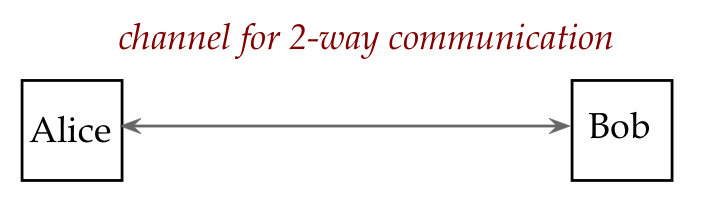
\includegraphics[width=4in]{notes/figs/n05/30channel.png}
        \caption{channel for 2-way communication}
        \label{fig:30channel}
    \end{figure}
    
    Example: mission control (Alice) to satellite (Bob) via radio waves (channel). Example: Headquarters (Alice) to regional bank office (Bob) over the internet (channel). Alice and Bob can use a one-time pad, which is unconditionally secure: They meet or securely-courier a shared book of random integers. This is not done using the channel but up front and securely. Subsequent text messages are encoded using these numbers, with a fresh page used for each message. Because the number patterns are never re-used, an adversary cannot gain any information statistically. And there are (incorrect) number patterns that will decode to valid text, making it impossible to judge whether a lucky guess is correct. The big downside of course is the inconvenience of sharing the one-time pads, and keeping them secure. Alternatively, Alice and Bob can use a short-term secret key, which is a sequence of random integers, and re-use that key for near-term messages: These keys can be created afresh periodically. The problem of sharing such keys is called key distribution. To share such keys without meeting, Alice and Bob use public-key cryptography. However, public-key cryptography relies on the hypothesis that the underlying mathematical problem cannot be easily solved: Factoring (large) integers, as in the RSA public-key system. The discrete log problem for elliptic-curve cryptography. As we will see in this course, a quantum computer can efficiently solve the former directly using Shor's algorithm, which can also used indirectly to solve $t$. The adversary: In any security solution, one must model the adversary. Often called the threat model. The primary attack we'll consider is "tapping into the line". Here, the attacker can receive the photons Alice sends. The attacker can either try to decipher, or both decipher and send photons along to Bob in order to evade detection. There are other, more sophisticated attacks we'll consider in a later module. Main ideas in quantum key distribution using the BB84 Protocol: BB84: Bennett and Brassard in 1984 (first such paper). BB84 aims to get a bit pattern securely from Alice to Bob. The protocol depends on the ability to send single qubits in particular states: In today's technology, the only practical flying qubit is a photon. Thus, the protocol relies on reliable single-photon transmission. Which is hard to do, but has been demonstrated over distances beyond $100 \mathrm{~km}$. The protocol also relies on being able to produce truly random bits: This is easy with quantum technology. For example, one simply feeds $|+\rangle$ qubits to a standard-basis measurement shown in Figure \ref{fig:31gate5}.
    
    \begin{figure}
        \centering
        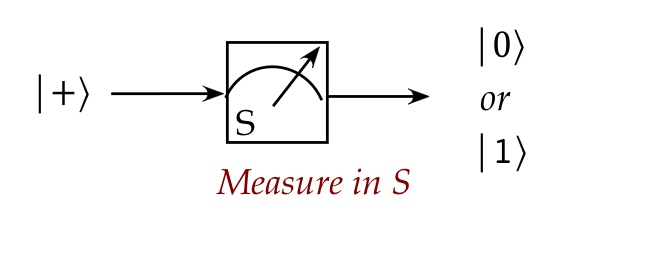
\includegraphics[width=4in]{notes/figs/n05/31gate5.png}
        \caption{Measure in $S$}
        \label{fig:31gate5}
    \end{figure}
    
    The protocol uses two channels in Figure \ref{fig:32bb}.

    \begin{figure}
        \centering
        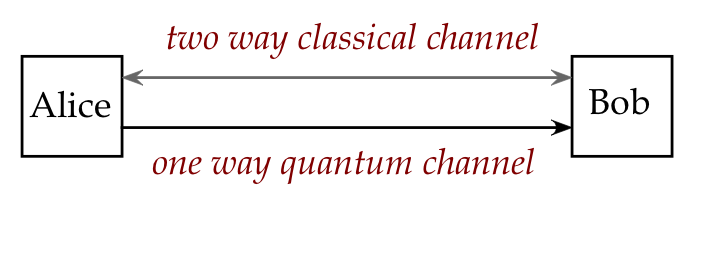
\includegraphics[width=4in]{notes/figs/n05/32bb.png}
        \caption{Two way vs One Way}
        \label{fig:32bb}
    \end{figure}
    
    The quantum channel transports qubits. The classical channel (which may have weaker security) is used for messages. Let's examine the steps in BB84: Step 1 (Alice): Alice creates a random bit string on her side shown in Figure \ref{fig:33bb2}.
    
    \begin{figure}
        \centering
        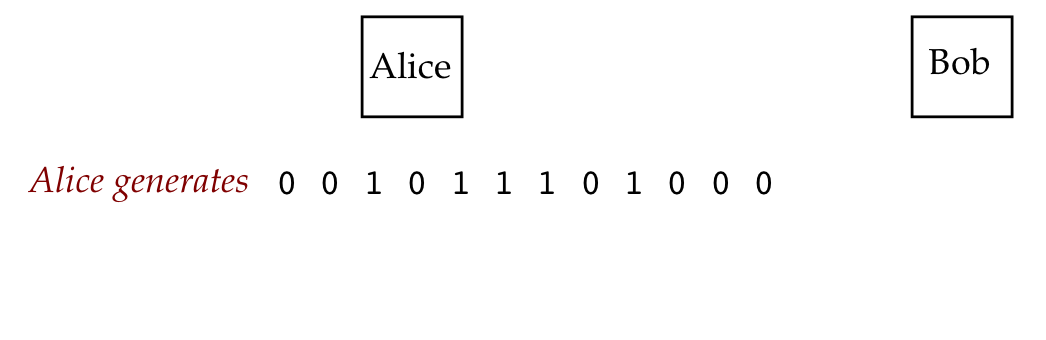
\includegraphics[width=4in]{notes/figs/n05/33bb2.png}
        \caption{Two way vs One Way}
        \label{fig:33bb2}
    \end{figure}
    
    We'll call these the classical potential key bits. Step 2 (Alice): Alice creates a random string using the letters "S" and " $\mathrm{H}^{\prime \prime}$, lining them up with the key bit pattern shown in Figure \ref{fig:34bb3}.
    
    \begin{figure}
        \centering
        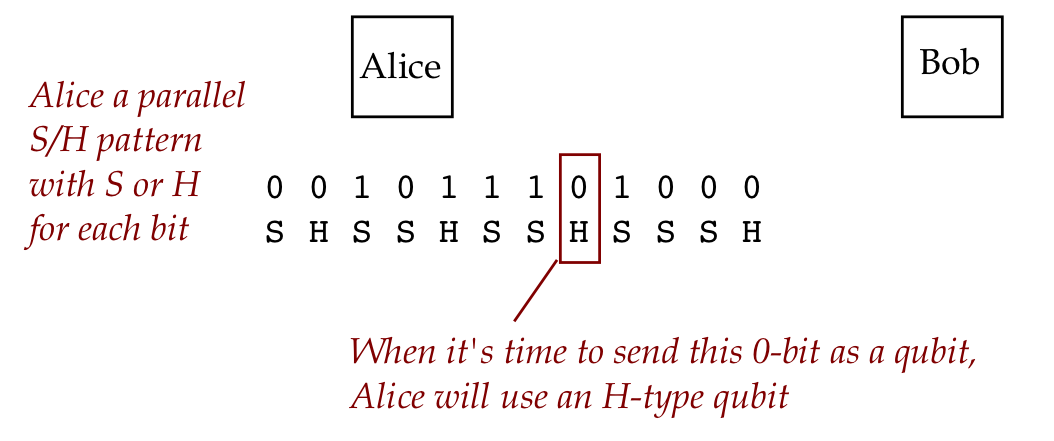
\includegraphics[width=4in]{notes/figs/n05/34bb3.png}
        \caption{Parallel $S/H$ pattern}
        \label{fig:34bb3}
    \end{figure}
    
    If a key bit is aligned with "S", she uses an S-type qubit for that bit. Otherwise, an "H" type qubit. Step 3 (Bob) is shown in Figure \ref{fig:35bb3a}.
    
    \begin{figure}
        \centering
        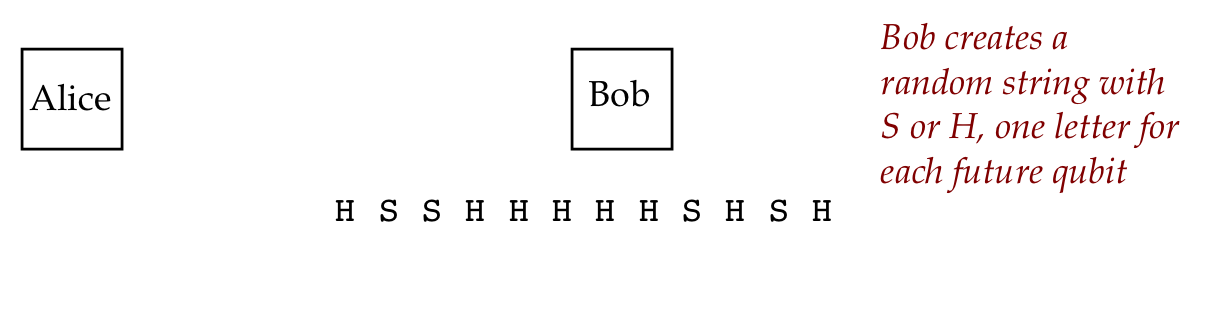
\includegraphics[width=4in]{notes/figs/n05/35bb3a.png}
        \caption{Random string}
        \label{fig:35bb3a}
    \end{figure}
   
   Bob's random string using the letters "S" and "H", will be used later in lining them up with the qubits that Alice will send. Step 4 (Alice): Alice then sends these as qubits, but using two different types of qubits: If a particular qubit has been designated an S-type qubit, then reference Figure \ref{fig:36bb4}.
   
    \begin{figure}
        \centering
        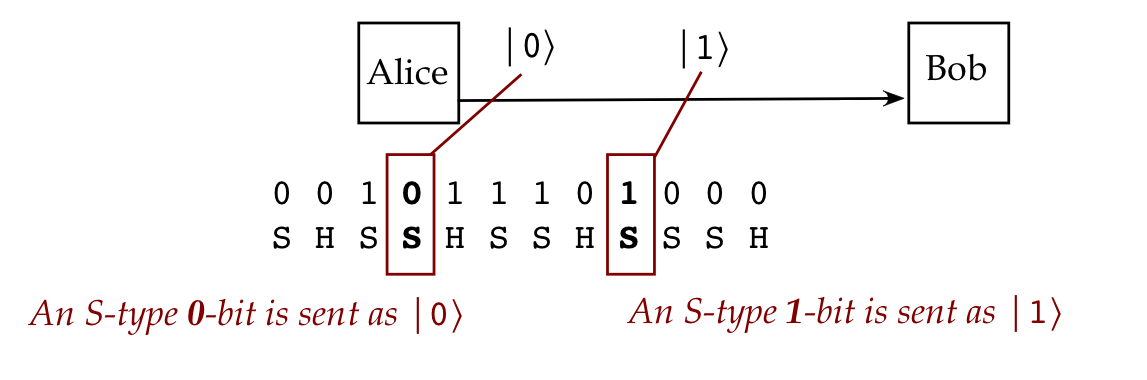
\includegraphics[width=4in]{notes/figs/n05/36bb4.png}
        \caption{$S$-type sent}
        \label{fig:36bb4}
    \end{figure}
    
    0 key bit $\Rightarrow$ send $|0\rangle$, 1 key bit $\Rightarrow$ send $|1\rangle$. If a particular qubit has been designated an H-type qubit, then reference Figure \ref{fig:37bb5}.
    
    \begin{figure}
        \centering
        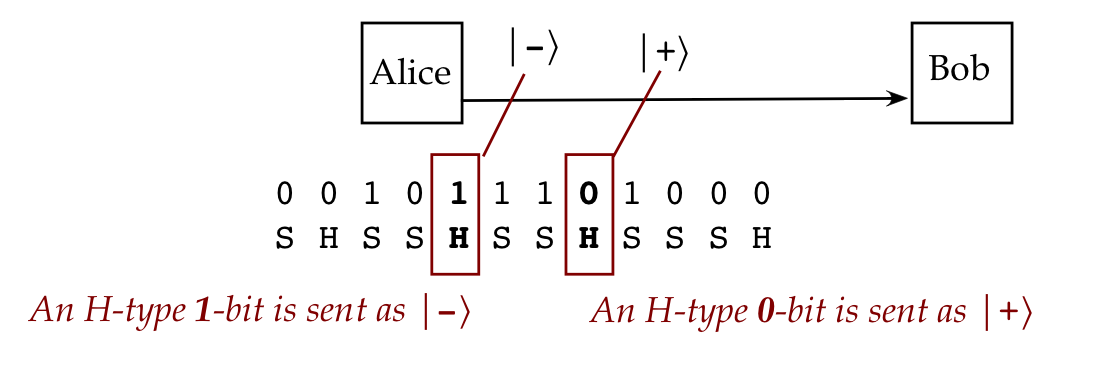
\includegraphics[width=4in]{notes/figs/n05/37bb5.png}
        \caption{$H$-type sent}
        \label{fig:37bb5}
    \end{figure}
    
    0 key bit $\Rightarrow$ send $|+\rangle$, 1 key bit $\Rightarrow$ send $|-\rangle$. In this manner, all the key bits get sent as $\mathrm{S}$ or $\mathrm{H}$ qubits. Step 5: (Bob) shown in Figure \ref{fig:38bb6}.
    
    \begin{figure}
        \centering
        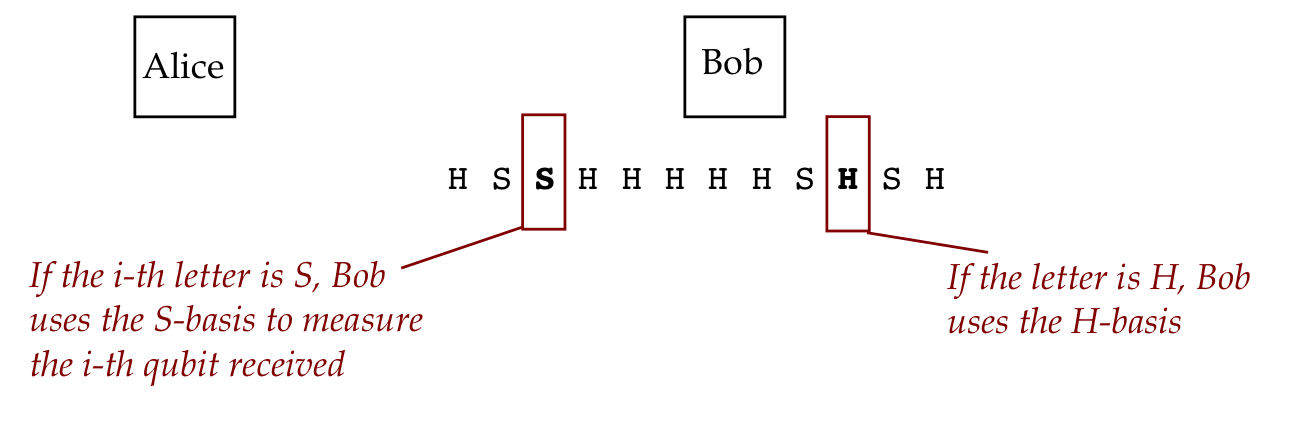
\includegraphics[width=4in]{notes/figs/n05/38bb6.png}
        \caption{$S$ or $H$ basis measurement}
        \label{fig:38bb6}
    \end{figure}
    
    Bob measures these qubits using two bases, depending on his "S-H" string. If the i-th letter is $S$, he uses the Standard-basis, $|0\rangle,|1\rangle$, to measure the i-th qubit. If he obtains $|0\rangle$, he infers 0 as the key bit. Otherwise $1.$ Otherwise he uses the Hadamard basis, $|+\rangle,|-\rangle$, If he obtains $|+\rangle$, he infers 0 as the key bit. Otherwise $1 .$ So, at the end of receiving all the qubits, Bob will have a key bit-string aligned with his S-H string: Step 6: (Alice and Bob) reference Figure \ref{fig:38bb6}.
    
    \begin{figure}
        \centering
        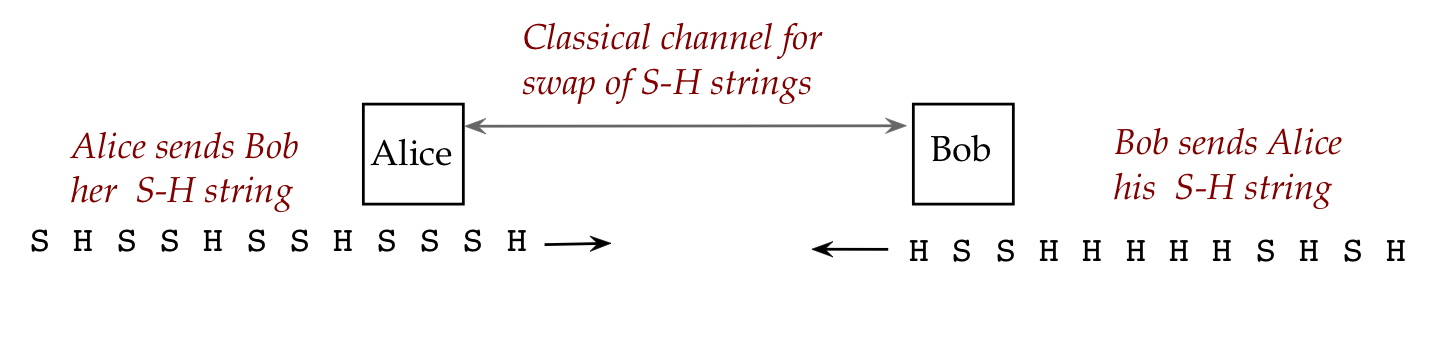
\includegraphics[width=4in]{notes/figs/n05/39bb7.png}
        \caption{Classical channel}
        \label{fig:38bb6}
    \end{figure}
    
    They use the classical channel to send each other their S-H strings. Step 7: (Alice and Bob) reference Figure \ref{fig:40bb8}.

    \begin{figure}
        \centering
        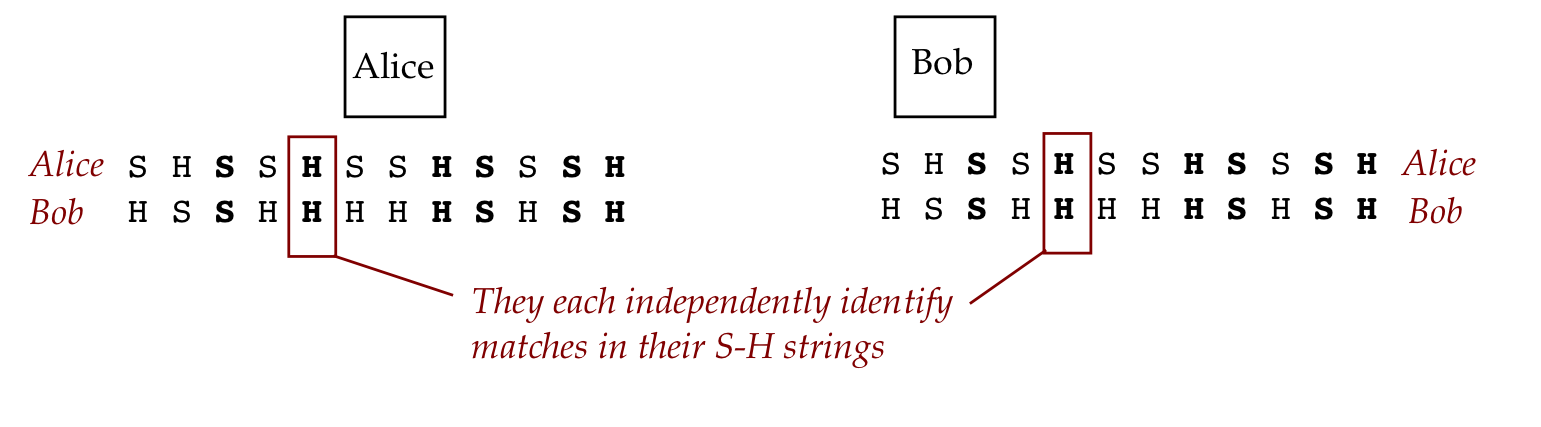
\includegraphics[width=4in]{notes/figs/n05/40bb8.png}
        \caption{Independently identify matches}
        \label{fig:40bb8}
    \end{figure}  
    
    They each identify the positions in their S-H strings where their letters match. Step 8: (Alice and Bob) reference Figure \ref{fig:41bb9}.
    
    \begin{figure}
        \centering
        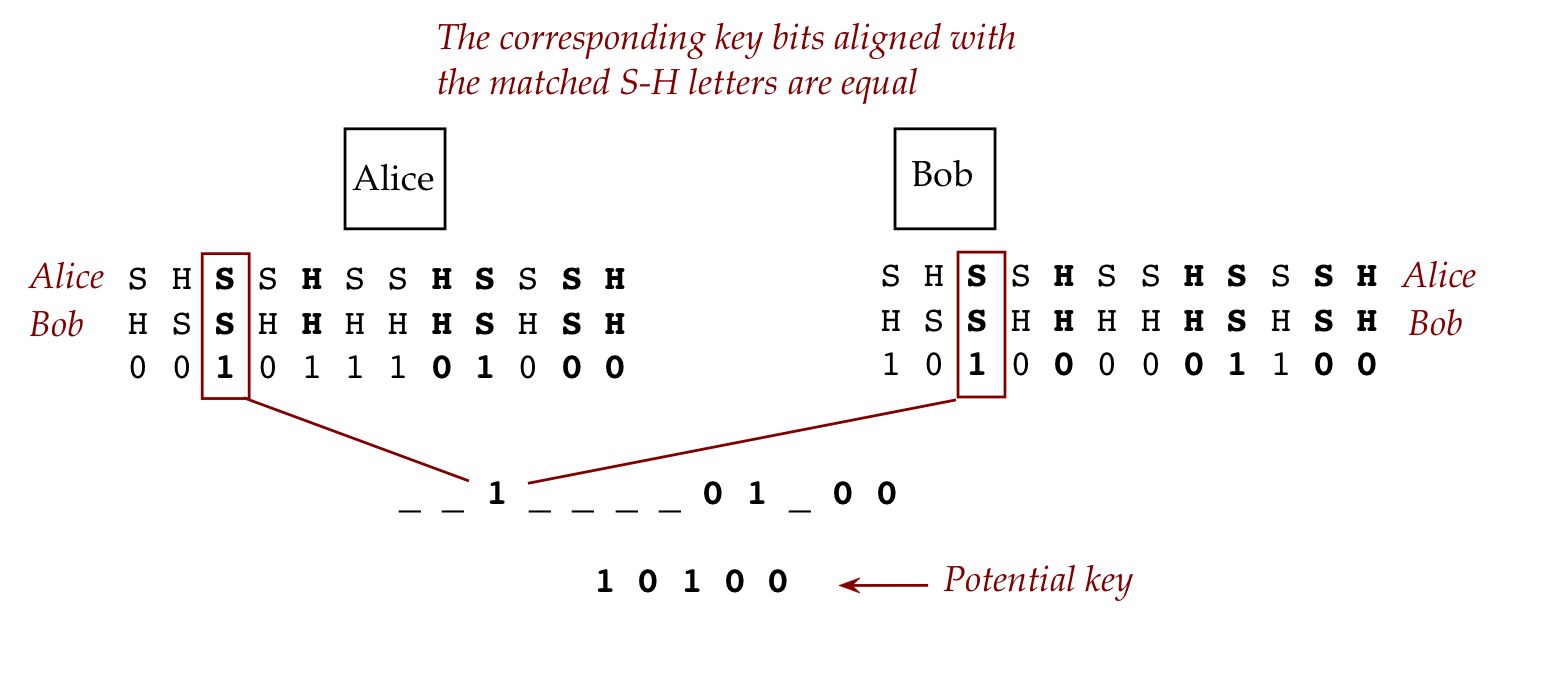
\includegraphics[width=4in]{notes/figs/n05/41bb9.png}
        \caption{Corresponding key bits aligned}
        \label{fig:41bb9}
    \end{figure} 
    
    The bits in the positions where S-H aligned are identical. These are the key bits. Note: the other bits may differ. Let's first examine correctness, assuming no attacker (Eve) is present. We'll consider two cases: When Alice and Bob use the same letter for a bit (S or H). When their letters are different. Case 1: same letter. Case 1(A): Alice uses S, Bob uses S reference Figure \ref{fig:42bb10}.
    
    \begin{figure}
        \centering
        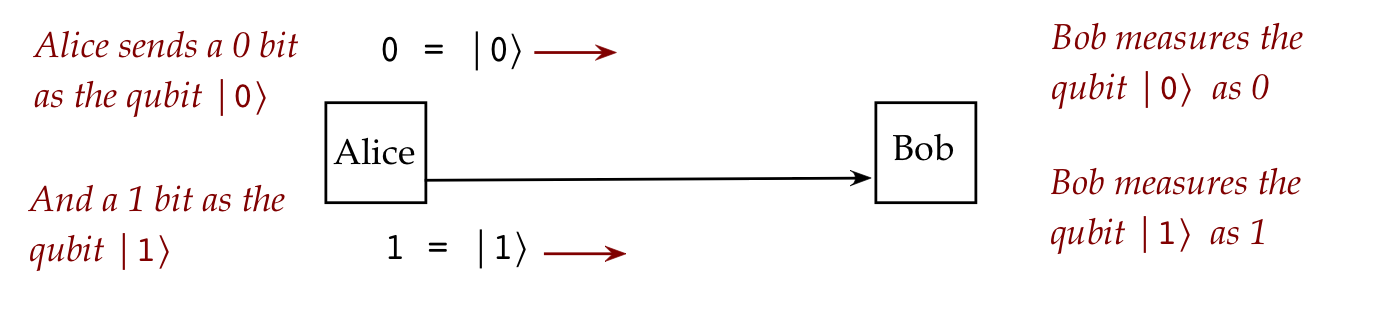
\includegraphics[width=4in]{notes/figs/n05/42bb10.png}
        \caption{Same Letter}
        \label{fig:42bb10}
    \end{figure} 
    
    If Alice has 0 as the classical bit, she sends $|0\rangle$. Bob uses S-basis and will see $|0\rangle$ with probability 1. Bob's bit is 0 , same as Alice's. If Alice has 1 as the classical bit, she sends $|1\rangle$. Bob will measure and see $|1\rangle$ with probability 1 . Bob's bit is 1 , same as Alice's Case 1(B): Alice uses H, Bob uses H. Reference Figure \ref{fig:43bb11}.
    
    \begin{figure}
        \centering
        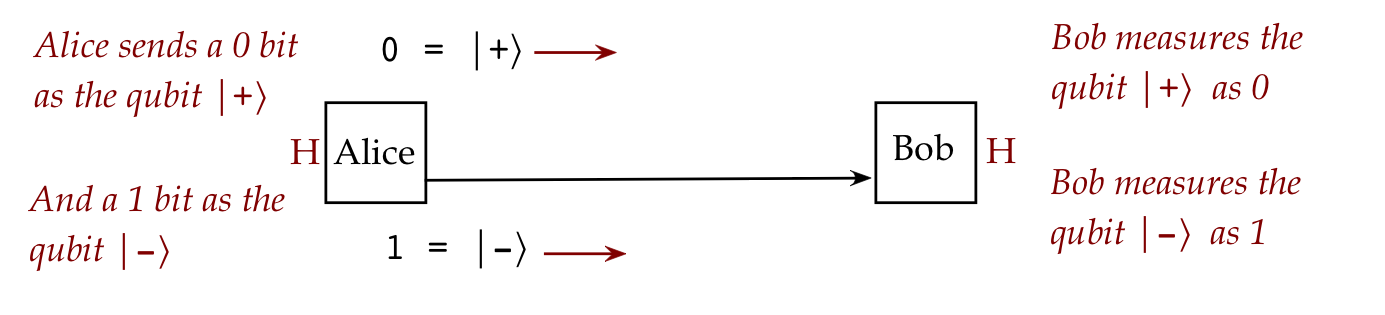
\includegraphics[width=4in]{notes/figs/n05/43bb11.png}
        \caption{Alice uses H, Bob uses H}
        \label{fig:43bb11}
    \end{figure} 
    
    If Alice has 0 as the classical bit, she sends $|+\rangle$. Bob uses $H$-basis and will see $|+\rangle$ with probability 1. Bob's bit is 0 , same as Alice's. If Alice has 1 as the classical bit, she sends $|-\rangle$. Bob will measure and see $|-\rangle$ with probability 1. Bob's bit is 1 , same as Alice's. Thus, in all cases when they use the same letter, the Bob correctly infers Alice's original classical bits with certainty. Case 2: different letter Case 2(A): Alice uses S, Bob uses H to measure. Reference Figure \ref{fig:44bb12}.
    
    \begin{figure}
        \centering
        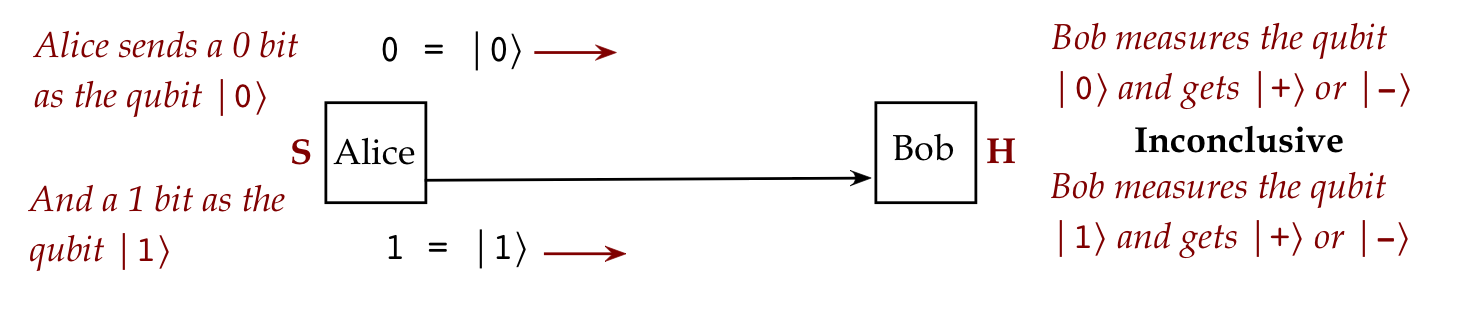
\includegraphics[width=4in]{notes/figs/n05/44bb12.png}
        \caption{Different letter}
        \label{fig:44bb12}
    \end{figure} 
    
    If Alice has 0 as the classical bit, she sends $|0\rangle$. Bob uses H-basis to measure. Bob gets $|+\rangle$ with probability $0.5$, Infers 0 with probability $0.5$. Bob gets $|-\rangle$ (infers 1 ) with probability $0.5$. If Alice has 1 as the classical bit, she sends $|1\rangle$. With H-basis measurement, Bob sees $|+\rangle$ with probability $0.5$, and infers 0. And with probability $0.5$, sees $|-\rangle$ and infers $1.$ To summarize: when their letter choices differ, Bob infers the correct bit with probability $0.5$. Thus, by throwing out the bits where they differed in $\mathrm{S}-\mathrm{H}$, the remaining bits agree exactly. Note: The actual classical bits were not transmitted. The S-H choices were exchanged after Bob performs all measurements. Let's now focus on Eve: Eve the eavesdropper, that is. What can Eve do? Reference Figure \ref{fig:45bb13}.
    
    \begin{figure}
        \centering
        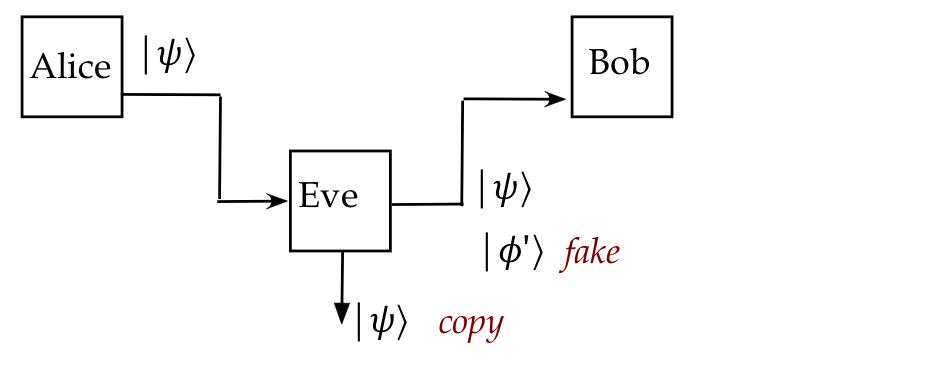
\includegraphics[width=4in]{notes/figs/n05/45bb13.png}
        \caption{Eve}
        \label{fig:45bb13}
    \end{figure} 
    
    Eve can try to copy (some or all of) the qubits by tapping the optical fiber. Eve can capture Alice's qubits and send fake qubits to Bob. Eve can pose as Alice to Bob (impersonate). Let's look at these one by one. We will later prove a simple but dramatic result: it is physically impossible, in general, to copy qubits. Reference Figure \ref{fig:46bb14}.
 
    \begin{figure}
        \centering
        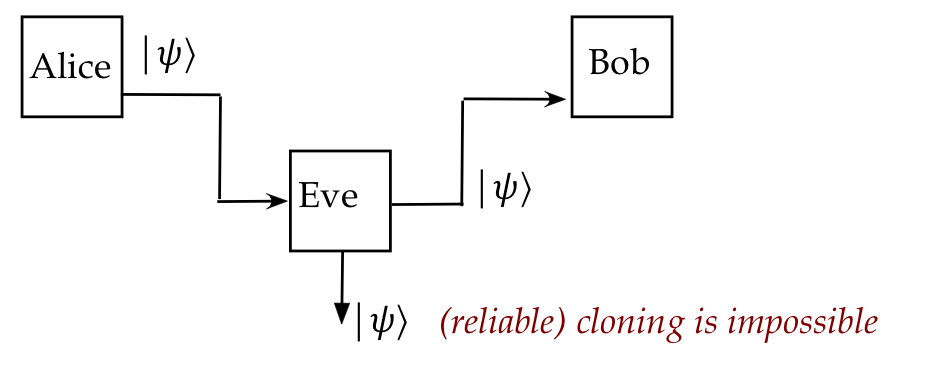
\includegraphics[width=4in]{notes/figs/n05/46bb14.png}
        \caption{No Cloning}
        \label{fig:46bb14}
    \end{figure}
    
    This is called the No-Cloning Theorem. There are some caveats, but in general, a clean accurate copy of a qubit can't be made without affecting the original. If Eve tries to intercept a few qubits, she'll have to guess which basis to use in measurement. Reference Figure \ref{fig:47bb15}.
    
    \begin{figure}
        \centering
        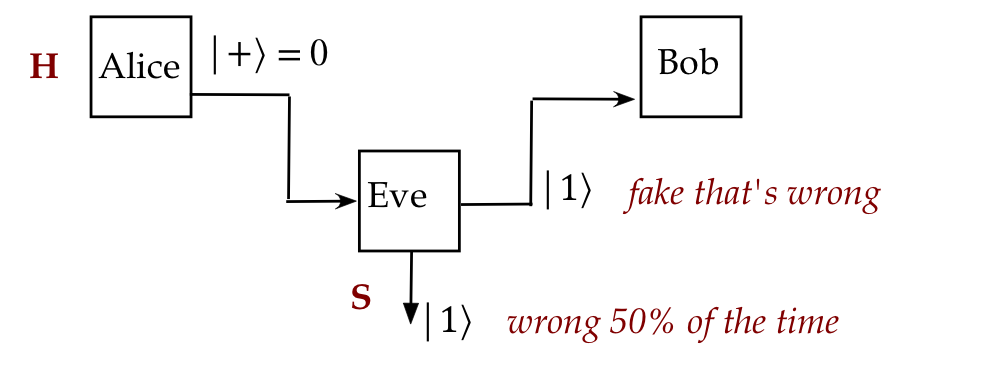
\includegraphics[width=4in]{notes/figs/n05/47bb15.png}
        \caption{Random Guessing}
        \label{fig:47bb15}
    \end{figure}  
    
    Which means she'll be wrong $50 \%$ of the time (with random guessing). These qubits will change state because of measurement. If she sends the changed qubits to Bob, then Alice and Bob can detect this (as we'll show below). What happens if Eve impersonates Alice? BB84 does not solve this problem. The assumption is that the Alice and Bob can somehow authenticate each other through the classical channel. An improvement: detecting Eve. Think of the agreed bits as the "good bits". Alice and Bob, through the classical channel, share $50 \%$ of their "good bits". This means the openly shared bits can't be used for the secret key. If Eve intercepted qubits and sent fake ones, then $50 \%$ of these supposedly good bits will differ between Alice and Bob. Eve will be caught. The remaining unshared good bits becomes the actual secret key to be used for future encryption.

\subsection{Phase equivalence in vectors}

    Consider these two vectors:
    
    $$
    \begin{aligned}
    |\psi\rangle &=\frac{\sqrt{2}}{\sqrt{3}}|0\rangle+\frac{1}{\sqrt{3}}|0\rangle \quad=\left[\begin{array}{c}
    \frac{\sqrt{2}}{\sqrt{3}} \\
    \frac{1}{\sqrt{3}}
    \end{array}\right] \\
    \left|\psi^{\prime}\right\rangle &=\left(\frac{2-\sqrt{2} i}{3}\right)|0\rangle+\left(\frac{\sqrt{2}-i}{3}\right)|1\rangle=\left[\begin{array}{c}
    \frac{2-\sqrt{2} i}{3} \\
    \frac{\sqrt{2}-i}{3}
    \end{array}\right]
    \end{aligned}
    $$
    
    Clearly, $|\psi\rangle$ and $\left|\psi^{\prime}\right\rangle$ are different vectors because there's no simplification of the components of $\left|\psi^{\prime}\right\rangle$ that will result in $|\psi\rangle$. Now consider the probability of obtaining $|0\rangle$ when each vector above is measured by in the 5 -basis (standard basis) shown in Figure \ref{fig:48phase}.
    
    \begin{figure}
        \centering
        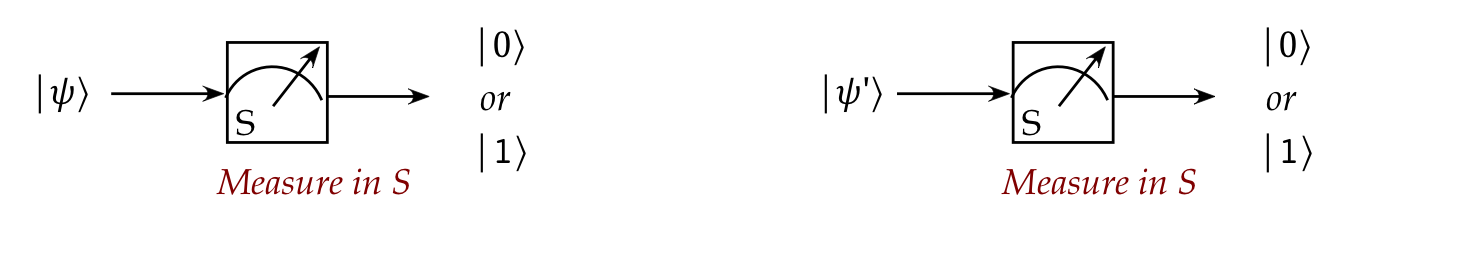
\includegraphics[width=4in]{notes/figs/n05/48phase.png}
        \caption{Measure in $S$}
        \label{fig:48phase}
    \end{figure}  
    
    When $|\psi\rangle$ is the input vector, the probability of obtaining $|0\rangle$ is:
    
    $$
    \operatorname{Pr}[|0\rangle]=\left|\frac{\sqrt{2}}{\sqrt{3}}\right|^{2}=\frac{2}{3}
    $$
    
    With $\left|\psi^{\prime}\right\rangle$ we get
    
    $$
    \operatorname{Pr}[|0\rangle]=\left|\frac{2-\sqrt{2} i}{3}\right|^{2}=\frac{2}{3}
    $$
    
    Both give the same results. Thus, experimentally, it is impossible to distinguish them with the S-basis measurement. Now suppose we define the number
    
    $$
    a=\frac{2}{\sqrt{6}}-i \frac{\sqrt{2}}{\sqrt{6}}
    $$
    
    The exercise below shows that
    
    $$
    \left|\psi^{\prime}\right\rangle=a|\psi\rangle
    $$
    
    and
    
    $$
    |a|^{2}=1
    $$
    
    Thus, we can write
    
    $$
    \left|\psi^{\prime}\right\rangle=\frac{a \sqrt{2}}{\sqrt{3}}|0\rangle+\frac{a}{\sqrt{3}}|0\rangle
    $$
    
    where the probability of obtaining $|0\rangle$ in S-basis is
    
    $$
    \operatorname{Pr}[|0\rangle]=\left|\frac{a \sqrt{2}}{\sqrt{3}}\right|^{2}=|a|^{2}\left|\frac{\sqrt{2}}{\sqrt{3}}\right|^{2}=\left|\frac{\sqrt{2}}{\sqrt{3}}\right|^{2}=\frac{2}{3}
    $$
    
    To clarify further, let's use
    
    $$
    |\psi\rangle=\alpha|0\rangle+\beta|1\rangle
    $$
    
    and
    
    $$
    \left|\psi^{\prime}\right\rangle=a|\psi\rangle=a \alpha|0\rangle+a \beta|1\rangle
    $$
    
    Then, $\left|\psi^{\prime}\right\rangle$
    
    $$
    \operatorname{Pr}[|0\rangle]=|a \alpha|^{2}=|a|^{2}|\alpha|^{2}=|\alpha|^{2}
    $$
    
    which is the same probability when using $|\psi\rangle$. Thus, for any complex number $a$ such that $|a|^{2}=1$, the two vectors $|\psi\rangle$ and $a|\psi\rangle$ are indistinguishable with regard to S-basis measurements. This will be true for any measurement basis. (See exercise below.) Thus, no experiment can reveal a measurable difference between $|\psi\rangle$ and $|\psi\rangle$. These two vectors are considered to represent the same quantum state and are called globally phase-equivalent vectors. There is another, commonly used way of looking at phase-equivalence: We know that any complex number $a$ can be written as
    
    $$
    a=r e^{i \theta}
    $$
    
    When $a$ has magnitude 1 , then $r=1$ and thus
    
    $$
    a=e^{i \theta}
    $$
    
    Now consider any vector $|\psi\rangle$ expressed in any basis $|v\rangle,\left|v^{\perp}\right\rangle$ :
    
    $$
    |\psi\rangle=\alpha|v\rangle+\beta\left|v^{\perp}\right\rangle
    $$
    
    and let
    
    $$
    \left|\psi^{\prime}\right\rangle=a|\psi\rangle=e^{i \theta}|\psi\rangle
    $$
    
    Then
    
    $$
    \left|\psi^{\prime}\right\rangle=e^{i \theta} \alpha|v\rangle+e^{i \theta} \beta\left|v^{\perp}\right\rangle
    $$
    
    Now when measured in the new $|v\rangle,\left|v^{\perp}\right\rangle$ basis, the probability of obtaining $|v\rangle$
    
    $$
    \operatorname{Pr}[|v\rangle]=\left|e^{i \theta} \alpha\right|^{2}=\left|e^{i \theta}\right|^{2}|\alpha|^{2}=|\alpha|^{2}
    $$
    
    Thus, no measurement can distinguish the two vectors: both represent the same quantum state. Now let's look at the concept of relative phase: Consider two vectors we're already familiar with:
    
    $$
    \begin{aligned}
    |+\rangle &=\frac{1}{\sqrt{2}}|0\rangle+\frac{1}{\sqrt{2}}|1\rangle \\
    |-\rangle &=\frac{1}{\sqrt{2}}|0\rangle-\frac{1}{\sqrt{2}}|1\rangle
    \end{aligned}
    $$
    
    At first glance, it may seem that the probability of obtaining $|0\rangle$ is the same for both vectors and they should therefore be considered indistinguishable. However, if we switch measurement to the H-basis, that is the $|+\rangle,|-\rangle$ basis, they are distinguishable. Thus, even though
    
    $$
    |-\rangle=\frac{1}{\sqrt{2}}|0\rangle+e^{i \pi} \frac{1}{\sqrt{2}}|1\rangle
    $$
    
    has one coefficient modified by an $e^{i \theta}$ term, it is distinguishable if we change the basis. In general we say that the two vectors
    
    $$
    \begin{aligned}
    |\psi\rangle &=\alpha|v\rangle+\beta\left|v^{\perp}\right\rangle \\
    \left|\psi^{\prime}\right\rangle &=\alpha|v\rangle+e^{i \theta} \beta\left|v^{\perp}\right\rangle
    \end{aligned}
    $$
    
    differ by relative phase and represent different quantum states.
    
    So, how do we know that a change of basis cannot distinguish two vectors in globally equivalent phases? Suppose $|\psi\rangle$ and $\left|\psi^{\prime}\right\rangle$ are two vectors such that
    
    $$
    \left|\psi^{\prime}\right\rangle=a|\psi\rangle
    $$
    
    Next, let's apply a change-of-basis matrix $M$ to $\left|\psi^{\prime}\right\rangle$
    
    $$
    M\left|\psi^{\prime}\right\rangle=M a|\psi\rangle=a M|\psi\rangle
    $$
    
    Thus, the constant $a$ multiplies into the changed coordinates and does not change the probabilities in the new basis.
    To summarize: Global phase does not matter and so, when there's a chance for simplification, we'll use this fact. Relative phase does matter and will, in fact, be exploited in algorithms, as we'll later see.

\subsection{Projective measurement}

    Let's start with recalling what we've learned about measurement so far: Measuring starts with: "what are we measuring?": The target of measuring is always a quantum state, a vector $|\psi\rangle$. In this module, we are focusing on the quantum state of a qubit. Later we will apply measurement to multiple qubits. A qubit measurement device, we've seen, is a basis $|v\rangle,\left|v^{\perp}\right\rangle$. The act of measurement involves: Express the state in terms of the measurement basis:
    
    $$
    |\psi\rangle=\alpha|v\rangle+\beta\left|v^{\perp}\right\rangle
    $$
    
    The outcomes of measurement will be one of the basis vectors $|v\rangle$ or $\left|v^{\perp}\right\rangle$. Which one occurs is probabilistically determined by nature, based on the coefficients $\alpha, \beta$ :
    
    $$
    \begin{aligned}
    \operatorname{Pr}[\text { observe }|v\rangle] &=|\alpha|^{2} \\
    \operatorname{Pr}\left[\text { observe }\left|v^{\perp}\right\rangle\right] &=|\beta|^{2}
    \end{aligned}
    $$
    
    We will now look at a broader theoretical framework for measurement based on projections: We'll still have a basis for measurement. But we'll use projection matrices on a state $|\psi\rangle$ to determine outcomes and probabilities. Why go through the extra trouble? Once we start to use projection operators (matrices), we'll be able to combine them smoothly using matrix properties. The theory so developed will naturally extend to including eigenvalues when projectors are combined. This is where Hermitian operators come in. The broader theory unifies quantum computing and mechanics. Recall projectors: In general, a projector for a vector $|v\rangle$ is an operator $P_{v}$ such that $P_{v}|\psi\rangle$ is along $|v\rangle$ for any $|\psi\rangle$. The operator is easily constructed: it's the outer-product created from $|v\rangle$ :
    
    $$
    P_{v}=|v\rangle\langle v|
    $$
    
    Let's revisit some examples: Example 1:
    
    $$
    \begin{aligned}
    &P_{0}=|0\rangle\langle 0|=\left[\begin{array}{l}
    1 \\
    0
    \end{array}\right]\left[\begin{array}{ll}
    1 & 0
    \end{array}\right]=\left[\begin{array}{ll}
    1 & 0 \\
    0 & 0
    \end{array}\right] \\
    &P_{1}=|1\rangle\langle 1|=\left[\begin{array}{l}
    0 \\
    1
    \end{array}\right]\left[\begin{array}{ll}
    0 & 1
    \end{array}\right]=\left[\begin{array}{ll}
    0 & 0 \\
    0 & 1
    \end{array}\right]
    \end{aligned}
    $$
    
    are the projectors for the basis vectors $|0\rangle,|1\rangle$. Example 2:
    
    $$
    \begin{aligned}
    &P_{+}=|+\rangle\langle+|=\left[\begin{array}{c}
    \frac{1}{\sqrt{2}} \\
    \frac{1}{\sqrt{2}}
    \end{array}\right]\left[\begin{array}{ll}
    \frac{1}{\sqrt{2}} & \frac{1}{\sqrt{2}}
    \end{array}\right]=\left[\begin{array}{cc}
    \frac{1}{2} & \frac{1}{2} \\
    \frac{1}{2} & \frac{1}{2}
    \end{array}\right] \\
    &P_{-}=|-\rangle\langle-|=\left[\begin{array}{r}
    \frac{1}{\sqrt{2}} \\
    -\frac{1}{\sqrt{2}}
    \end{array}\right]\left[\begin{array}{ll}
    \frac{1}{\sqrt{2}} & -\frac{1}{\sqrt{2}}
    \end{array}\right]=\left[\begin{array}{cc}
    \frac{1}{2} & -\frac{1}{2} \\
    -\frac{1}{2} & \frac{1}{2}
    \end{array}\right]
    \end{aligned}
    $$
    
    are the projectors for the basis vectors $|+\rangle,|-\rangle$. Now let's apply projectors to measurement: When we say "apply", we mean to a current qubit state $|\psi\rangle$. We will do four things when applying projective measurement to a vector $|\psi\rangle$ : 1. Identify the projectors of interest. 2. Compute the resulting projections, one for each projector $P$ :
    
    $$
    \left|\psi_{P}\right\rangle=P|\psi\rangle
    $$
    
    3. Compute the squared magnitude of the resulting vectors:
    
    $$
    \left.\left.|| \psi_{P}\right\rangle\left.\right|^{2}=|P| \psi\right\rangle\left.\right|^{2}
    $$
    
    This will necessarily be less than or equal to 1 , and will be the probability of obtaining the normalized-projection (next). 4. Compute the normalized projections:
    
    $$
    \left|\psi_{N}\right\rangle=\frac{\left|\psi_{P}\right\rangle}{\left.|| \psi_{P}\right\rangle \mid}=\frac{P|\psi\rangle}{|P| \psi\rangle \mid}
    $$
    
    Each such vector is one of the possible outcomes of measurement. Projective measurement for a single qubit via an example: Let's use the S-basis $|0\rangle,|1\rangle$ for measuring
    
    $$
    |\psi\rangle=\alpha|0\rangle+\beta|1\rangle
    $$
    
    Step 1: Identify the projectors of interest. Here, there are two, one for each basis vector:
    
    $$
    \begin{aligned}
    &P_{0}=\left[\begin{array}{ll}
    1 & 0 \\
    0 & 0
    \end{array}\right] \\
    &P_{1}=\left[\begin{array}{ll}
    0 & 0 \\
    0 & 1
    \end{array}\right]
    \end{aligned}
    $$
    
    Step 2: compute the projected vectors
    
    $$
    \begin{aligned}
    &\left|\psi_{P_{0}}\right\rangle=P_{0}|\psi\rangle=\left[\begin{array}{ll}
    1 & 0 \\
    0 & 0
    \end{array}\right]\left[\begin{array}{c}
    \alpha \\
    \beta
    \end{array}\right]=\left[\begin{array}{l}
    \alpha \\
    0
    \end{array}\right]=\alpha|0\rangle \\
    &\left|\psi_{P_{1}}\right\rangle=P_{1}|\psi\rangle=\left[\begin{array}{ll}
    0 & 0 \\
    0 & 1
    \end{array}\right]\left[\begin{array}{l}
    \alpha \\
    \beta
    \end{array}\right]=\left[\begin{array}{l}
    0 \\
    \beta
    \end{array}\right]=\beta|1\rangle
    \end{aligned}
    $$
    
    Step 3: compute the squared magnitude of each projection:
    
    $$
    \begin{aligned}
    &\left.\left.\left.\left.|| \psi_{P_{0}}\right\rangle\left.\right|^{2}=|\alpha| 0\right\rangle\left.\right|^{2}=\langle\alpha \mid 0\rangle|\alpha| 0\right\rangle\right\rangle=\alpha^{*} \alpha\langle 0 \mid 0\rangle=|\alpha|^{2} \\
    &\left.\left.\left.\left.|| \psi_{P_{1}}\right\rangle\left.\right|^{2}=|\beta| 1\right\rangle\left.\right|^{2}=\langle\beta \mid 1\rangle|\beta| 1\right\rangle\right\rangle=\beta^{*} \beta\langle 1 \mid 1\rangle=|\beta|^{2}
    \end{aligned}
    $$
    
    Step 4: compute the normalized projections:
    
    $$
    \begin{aligned}
    \left|\psi_{N_{0}}\right\rangle &=\frac{P_{0}|\psi\rangle}{\left.\left|P_{0}\right| \psi\right\rangle \mid}=\frac{\alpha|0\rangle}{|\alpha|} \\
    \left|\psi_{N_{1}}\right\rangle &=\frac{P_{1}|\psi\rangle}{\left.\left|P_{1}\right| \psi\right\rangle \mid}=\frac{\beta|1\rangle}{|\beta|}
    \end{aligned}
    $$
    
    Now analyze what happens in measurement: The two possible outcomes of measurement are the normalized projections:
    
    $$
    \begin{aligned}
    \left|\psi_{N_{0}}\right\rangle &=\frac{\alpha|0\rangle}{|\alpha|} \\
    \left|\psi_{N_{1}}\right\rangle &=\frac{\beta|1\rangle}{|\beta|}
    \end{aligned}
    $$
    
    They each occur with probabilities (Step 3)
    
    $$
    \begin{aligned}
    &\operatorname{Pr}\left[\text { observe } \psi_{N_{0}}\right]=|\alpha|^{2} \\
    &\operatorname{Pr}\left[\text { observe } \psi_{N_{1}}\right]=|\beta|^{2}
    \end{aligned}
    $$
    
    There is one matter to clear up: In the earlier approach to measurement in S-basis, the outcomes were $|0\rangle$ or |1). But the projective approach has outcomes
    
    $$
    \frac{\alpha|0\rangle}{|\alpha|} \quad \text { or } \frac{\beta|1\rangle}{|\beta|}
    $$
    
    Do the two approaches differ in outcomes? They are in fact the same because of global-phase equivalence:
    
    $$
    \frac{\alpha}{|\alpha|}|0\rangle=|0\rangle
    $$
    
    because
    
    $$
    \left|\frac{\alpha}{|\alpha|}\right|=\frac{|\alpha|}{|\alpha|}=1
    $$
    
    Knowing this, we'll of course write the simpler $|0\rangle,|1\rangle$ as outcomes. Let's summarize by going to general n-dimensional space (since we'll be getting there soon): Suppose $\left|v_{1}\right\rangle,\left|v_{2}\right\rangle, \ldots,\left|v_{n}\right\rangle$ represents a measurement basis. Next, suppose $|\psi\rangle$ is an n-dimensional complex vector representing a quantum state of some quantum object. The four steps (with simplified subscripts) are 1. Identify the projectors for the basis:
    
    $$
    P_{i}=\left|v_{i}\right\rangle\left\langle v_{i}\right|
    $$
    
    2. Compute each projected vector
    
    $$
    \left|\psi_{P_{i}}\right\rangle=P_{i}|\psi\rangle
    $$
    
    3. Compute the squared magnitude of each projection:
    
    $$
    \left.|| \psi_{P_{i}}\right\rangle\left.\right|^{2}
    $$
    
    as the probability of seeing the i-th normalized projection. 4. Compute each normalized projection (each potential outcome):
    
    $$
    \left|\psi_{N_{i}}\right\rangle=\frac{\left|\psi_{P_{i}}\right\rangle}{\left.|| \psi_{P_{i}}\right\rangle \mid}
    $$
    
    Then we have the outcomes and their probabilities: Outcome $\left|\psi_{N_{\mathrm{i}}}\right\rangle$ occurs with probability ||$\left.\psi_{P_{\mathrm{i}}}\right\rangle\left.\right|^{2}$ Lastly, let's point out that we could have used Dirac notation when working with the projectors: (Step 1) The two projectors:
    
    $$
    \begin{aligned}
    &P_{0}=|0\rangle\langle 0| \\
    &P_{1}=|1\rangle\langle 1|
    \end{aligned}
    $$
    
    (Step 2) The projected vectors:
    
    $$
    \begin{aligned}
    &\left|\psi_{P_{0}}\right\rangle=P_{0}|\psi\rangle=|0\rangle\langle 0|(\alpha|0\rangle+\beta|1\rangle)=\alpha| 0\rangle \\
    &\left|\psi_{P_{1}}\right\rangle=P_{1}|\psi\rangle=|1\rangle\langle 1|(\alpha|0\rangle+\beta|1\rangle)=\beta| 1\rangle
    \end{aligned}
    $$

\subsection{Hermitians and measurement}

    Hermitian operators play a central role in measurement, and purpose of this section is to connect the dots between the projector approach and Hermitians. Let's start by recall some facts about Hermitians: A Hermitian operator $A$ satisfies $A^{\dagger}=A$. Hermitian operators have real eigenvalues $\lambda_{1}, \lambda_{2}, \ldots, \lambda_{n}$. The eigenvectors of a Hermitian operator, $\left|\phi_{1}\right\rangle,\left|\phi_{2}\right\rangle, \ldots,\left|\phi_{n}\right\rangle$, form an orthonormal basis. By the spectral theorem, we can write
    
    $$
    A=\sum_{i} \lambda_{i}\left|\phi_{i}\right\rangle\left\langle\phi_{i}\right|
    $$
    
    which is a real-linear combination of the projectors $P_{i}=\left|\phi_{i}\right\rangle\left\langle\phi_{i}\right|$ formed from the eigenvectors. We can think of this result as "Did you know that a Hermitian can be decomposed into a linear combination of its eigenvector projectors, where the coefficients are the eigenvalues?" Now let's go the other way: from projectors to Hermitians. Suppose we have an orthonormal basis $\left|v_{1}\right\rangle,\left|v_{2}\right\rangle, \ldots,\left|v_{n}\right\rangle$. And suppose $\gamma_{1}, \gamma_{2}, \ldots, \gamma_{n}$ are any distinct real numbers. Then, the linear combination of projectors
    
    $$
    \sum_{i} \gamma_{i} P_{v_{i}}=\sum_{i} \gamma_{i}\left|v_{i}\right\rangle\left\langle v_{i}\right|
    $$
    
    is a Hermitian operator. (We proved this in Module 2.) Moreover, this operator has eigenvalues $\gamma_{1}, \gamma_{2}, \ldots, \gamma_{n}$ and associated eigenvectors $\left|v_{1}\right\rangle,\left|v_{2}\right\rangle, \ldots,\left|v_{n}\right\rangle$. How do we know this?
    
    $$
    \left(\sum_{j} \gamma_{j}\left|v_{j}\right\rangle\left\langle v_{j}\right|\right)\left|v_{i}\right\rangle=\gamma_{i}\left|v_{i}\right\rangle\left\langle v_{i}|| v_{i}\right\rangle=\gamma_{i}\left|v_{i}\right\rangle
    $$
    
    That is, the combination of projectors has eigenvector $\left|v_{i}\right\rangle$ with corresponding eigenvalue $\gamma_{i}$. Let's go a step further and see this in an example: Here, we pick the numbers $\gamma_{1}, \gamma_{2}, \ldots, \gamma_{n}$. In 2D, we'll pick, say $\gamma_{1}=2, \gamma_{2}=3$. Consider the S-basis and let
    
    $$
    A=\gamma_{1}|0\rangle\left\langle 0\left|+\gamma_{2}\right| 1\right\rangle\langle 1|=2\left[\begin{array}{ll}
    1 & 0 \\
    0 & 0
    \end{array}\right]+3\left[\begin{array}{ll}
    0 & 0 \\
    0 & 1
    \end{array}\right]=\left[\begin{array}{ll}
    2 & 0 \\
    0 & 3
    \end{array}\right]
    $$
    
    Then, $A$ is Hermitian with eigenvalues 2 and $3 .$ Think of this artificially constructed Hermitian as "packaging" all the projectors together in a way that lets the spectral decomposition recover the individual projectors. The Hermitian also includes eigenvalues, one per projector. How does any of this matter? Recall: we've said that the outcome of a measurement is one of the basis vectors involved. There is in fact another outcome: the associated eigenvalue: For a Hermitian that's derived from an actual physical quantum object, there are two outcomes: The eigenvector that will be the resulting state. The associated eigenvalue. In real physical devices, the associated eigenvalue (a real number) is a physical quantity that's observable, like energy or frequency. Reference Figure \ref{fig:49qubit5d}.
    
    \begin{figure}
        \centering
        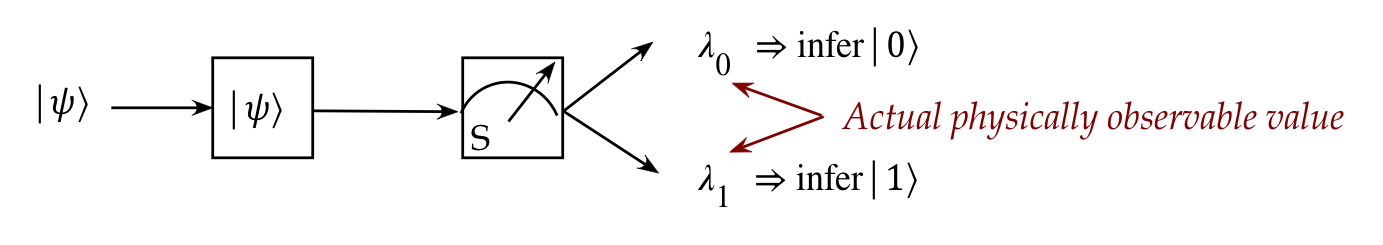
\includegraphics[width=4in]{notes/figs/n05/49qubit5d.png}
        \caption{Physically observable value}
        \label{fig:49qubit5d}
    \end{figure} 
    
    Thus, the eigenvalue matters in physical models because it is the quantifiable output that a device reports. But in quantum computing, such eigenvalues play no role. We only care about the resulting eigenvectors. Nonetheless, we will use the Hermitian formulation because: When you later encounter theory it will be in this form, as we'll see in the next section. Because Hermitian matrices package projectors, the theory develops powerful ways to combine Hermitians, as we'll see.

\subsection{The Hermitian sandwich}

    Recall that an eigenvalue is one of the measurement outcomes in a physical experiment. Each repetition of an experiment will result in one of the eigenvalues appearing, according to the probabilities involved: Suppose $|\psi\rangle$ is a state vector. Next, let the Hermitian operator $A$ represent a measurement. Suppose that $A$ has eigenvectors $\left|\phi_{1}\right\rangle,\left|\phi_{2}\right\rangle, \ldots,\left|\phi_{n}\right\rangle$, with corresponding eigenvalues $\lambda_{1}, \lambda_{2}, \ldots, \lambda_{n}$. Then, we know that: The resulting state after measurement will be one of: $\left|\phi_{1}\right\rangle,\left|\phi_{2}\right\rangle, \ldots,\left|\phi_{n}\right\rangle$. If the physical state $\left|\phi_{i}\right\rangle$ results, the physical quantity $\lambda_{i}$ will be observed. Alternatively: if $\lambda_{i}$ is observed, one concludes that the resulting state is $\left|\phi_{i}\right\rangle$. Let's focus on which $\lambda_{i}$ 's we see in several repetitions of measuring the original $|\psi\rangle$. For example, we might see, Trial #1: $\lambda_{3}$, Trial #2: $\lambda_{7}$, Trial #3: $\lambda_{1}$, Trial #4: $\lambda_{3}$. We are interested now in the mean (average) eigenvalue obtained:
    
    $$
    \frac{\lambda_{3}+\lambda_{7}+\lambda_{1}+\lambda_{3}+\ldots}{\text { number of trials }}
    $$
    
    This is from an experiment with repeated trials. We'd like to calculate this exactly using the probabilities from the model. For this, we use the expected-value calculation. If $p_{i}=$ probability of obtaining $\lambda_{i}$ then the mean is
    
    $$
    \sum_{i} \lambda_{i} p_{i}
    $$
    
    Such an expected value and is often written as:
    
    $$
    \langle\lambda\rangle=\sum_{i} \lambda_{i} p_{i}
    $$
    
    where $\lambda$ is a random variable representing the possible values $\lambda_{1}, \ldots, \lambda_{n}$. Now, the probabilities depend on the particular state $|\psi\rangle$. Let's write $|\psi\rangle$ in terms of the measurement basis
    
    $$
    |\psi\rangle=\alpha_{1} \phi_{1}+\ldots+\alpha_{n} \phi_{n}
    $$
    
    Then
    
    $$
    p_{i}=\left|\alpha_{i}\right|^{2}
    $$
    
    Using the sandwich: Let's compute $\langle\psi|A| \psi\rangle$ :
    
    $$
    \begin{aligned}
    \langle\psi|A| \psi\rangle &=\left\langle\sum_{i} \alpha_{i}^{*}\left\langle\phi_{i}|| \sum_{j} \lambda_{j} \mid \phi_{j}\right\rangle\left\langle\phi_{j}|| \sum_{k} \alpha_{k} \mid \phi_{k}\right\rangle\right\rangle \\
    &=\left\langle\sum_{i} \alpha_{i}^{*}\left\langle\phi_{i}|| \sum_{j} \lambda_{j} \alpha_{j} \mid \phi_{j}\right\rangle\right\rangle \\
    &=\sum_{i} \alpha_{i}^{*} \alpha_{i} \lambda_{i}\left\langle\phi_{i} \mid \phi_{i}\right\rangle \\
    &=\sum_{i} \lambda_{i}\left|\alpha_{i}\right|^{2} \\
    &=\langle\lambda\rangle
    \end{aligned}
    $$
    
    Thus
    
    $$
    \langle\lambda\rangle=\langle\psi|A| \psi\rangle
    $$
    
    Since each expectation depends on the state, we corld make that explicit in the notation:
    
    $$
    \left\langle\lambda_{\psi}\right\rangle=\langle\psi|A| \psi\rangle
    $$
    
    The sandwich has other uses: For example, one can compute the expected value of $\lambda_{\psi}^{2}$ (called the 2 nd moment).
    
    $$
    \left\langle\lambda_{\psi}^{2}\right\rangle=\left\langle\psi\left|A^{2}\right| \psi\right\rangle
    $$
    
    where $A^{2}$ is the operator applied twice (matrix multiplication). And from there, the variance:
    
    $$
    \operatorname{var}(\lambda)=\left\langle\psi\left|A^{2}\right| \psi\right\rangle-\langle\psi|A| \psi\rangle^{2}
    $$
    
    One can then reason about such statistics with multiple operators and their covariance, and analyze them over all possible $|\psi\rangle$. Dne such famous result: Heisenberg's uncertainty principle.

\subsection{The projector sandwich}

    Let's return briefly to the three steps in projective measurement: 1. Compute each projected vector
    
    $$
    \left|\psi_{P_{i}}\right\rangle=P_{i}|\psi\rangle
    $$
    
    2. Compute the squared magnitude of each projection:
    
    $$
    \left.\left.\| \psi_{P_{i}}\right\rangle\left.\right|^{2}=\left|P_{i}\right| \psi\right\rangle\left.\right|^{2}
    $$
    
    as the probability of seeing the i-th normalized projection. 3. Compute each normalized projection (each potential outcome):
    
    $$
    \left|\psi_{N_{i}}\right\rangle=\frac{\left|\psi_{N_{i}}\right\rangle}{\left.\| \psi_{P_{i}}\right\rangle \mid}=\frac{P_{i}|\psi\rangle}{\left.\left|P_{i}\right| \psi\right\rangle \mid}
    $$
    
    It is often convenient to use sandwich notation for the second step: First observe:
    
    $$
    \begin{aligned}
    \left.\left|P_{i}\right| \psi\right\rangle\left.\right|^{2} &=\left\langle P_{i} \psi \mid P_{i} \psi\right\rangle & & \text { Squared magritudes imner product } \\
    &=\left\langle\psi\left|P_{i}^{\dagger} P_{i}\right| \psi\right\rangle & & \text { Conjugate when moving accross } \\
    &=\left\langle\psi\left|P_{i} P_{i}\right| \psi\right\rangle & & P_{\text {is }} \text { is Hermitian } \\
    &=\left\langle\psi\left|P_{i}\right| \psi\right\rangle & & P_{1} \text { is idempotent }
    \end{aligned}
    $$
    
    Thus, we can write the second step as:
    
    $$
    \left.|| \psi_{P_{\mathrm{t}}}\right\rangle\left.\right|^{2}=\left\langle\psi\left|P_{i}\right| \psi\right\rangle
    $$
    
    And the third step as:
    
    $$
    \left|\psi_{N_{\mathrm{i}}}\right\rangle==\frac{P_{i}|\psi\rangle}{\sqrt{\left\langle\psi\left|P_{i}\right| \psi\right\rangle}}
    $$

\subsection{Matrix calculations with Dirac notation}

    Let's revisit the $X$ operator that "flipped" a qubit:
    
    $$
    X|0\rangle=\left[\begin{array}{ll}
    0 & 1 \\
    1 & 0
    \end{array}\right]\left[\begin{array}{l}
    1 \\
    0
    \end{array}\right]=\left[\begin{array}{l}
    0 \\
    1
    \end{array}\right]=|1\rangle
    $$
    
    Notice that: In applying the operator, we wrote the operator in matrix form, then wrote the $|0\rangle$ vector as a column vector. There is an alternate way that uses Dirac notation: First express the operator using outer products:
    
    $$
    X=|0\rangle\langle 1|+| 1\rangle\langle 0|
    $$
    
    To see why:
    
    $$
    \begin{aligned}
    |0\rangle\langle 1|+| 1\rangle\langle 0| &=\left[\begin{array}{l}
    1 \\
    0
    \end{array}\right]\left[\begin{array}{ll}
    0 & 1
    \end{array}\right.\\
    &=\left[\begin{array}{ll}
    0 & 1 \\
    0 & 0
    \end{array}\right]+\\
    &=\left[\begin{array}{ll}
    0 & 1 \\
    1 & 0
    \end{array}\right] \\
    &=X
    \end{aligned}
    $$
    
    Then apply:
    
    $$
    X|0\rangle=(|0\rangle\langle 1|+| 1\rangle\langle 0|)|0\rangle=|0\rangle\langle 1|| 0\rangle+|1\rangle\langle 0|| 0\rangle=\langle 1 \mid 0\rangle|0\rangle+\langle 0 \mid 0\rangle|1\rangle=|1\rangle
    $$
    
    This exploits the simplifications possible with orthonormal vectors when most inner products evaluate to $0 .$ It is not always the case that the Dirac approach will simplify, but we will see cases where it turns out to be simpler. This is the case when we work with muliple qubits where the matrix sizes are large. Let's apply $X$ to a general vector $|\psi\rangle=\alpha|0\rangle+\beta|1\rangle$
    
    $$
    \begin{aligned}
    X|\psi\rangle &=(|0\rangle\langle 1|+| 1\rangle\langle 0|)(\alpha|0\rangle+\beta|1\rangle) \\
    &=\beta\langle 1 \mid 1\rangle|0\rangle+\alpha\langle 0 \mid 0\rangle|1\rangle \\
    &=\beta|0\rangle+\alpha|1\rangle
    \end{aligned}
    $$
    
    as expected. 
    
\subsection{Stern-Gerlach explained}
    
    Let's revisit two Stern-Gerlach experiments from Module 1 that will be sufficient to outline the explanation: First reference Figure \ref{fig:50sg3}.
    
    \begin{figure}
        \centering
        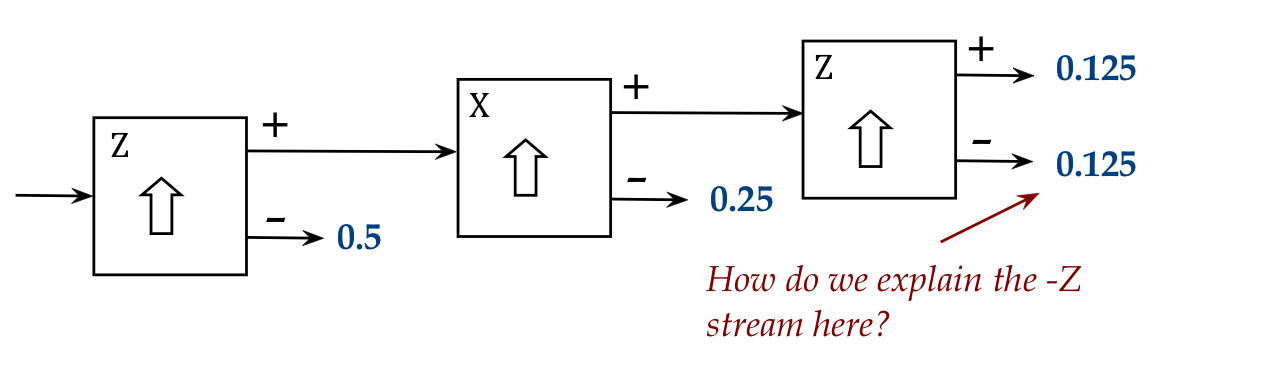
\includegraphics[width=4in]{notes/figs/n05/50sg3.png}
        \caption{-$Z$ stream}
        \label{fig:50sg3}
    \end{figure} 
    
    And then
    
    \begin{figure}
        \centering
        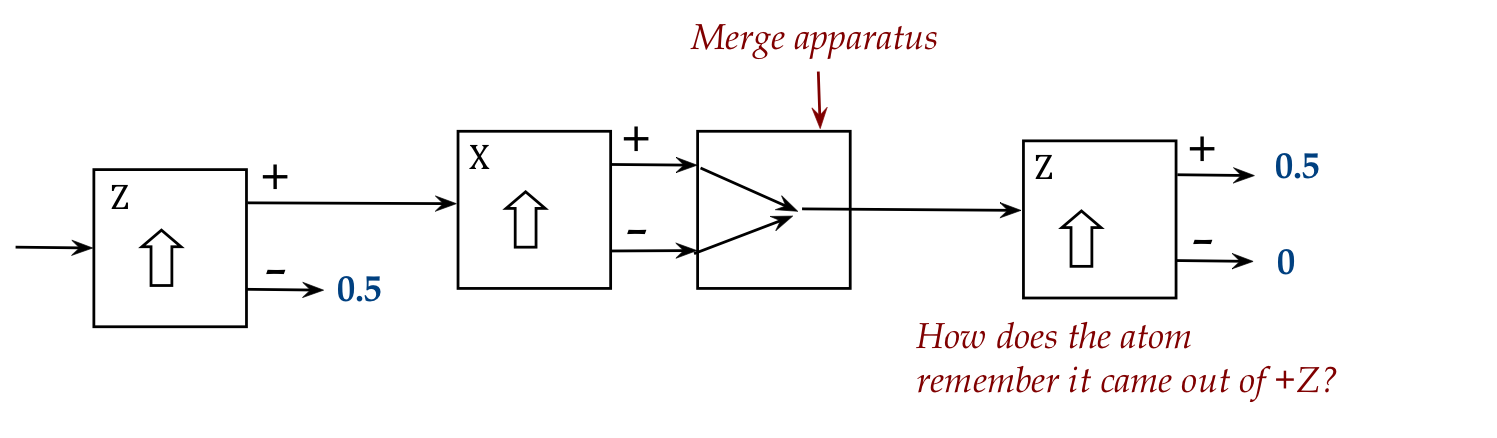
\includegraphics[width=4in]{notes/figs/n05/51sg4.png}
        \caption{Merge}
        \label{fig:51sg4}
    \end{figure}
    
    The quantum framework: We model the state of an atom as a $2 \mathrm{D}$ vector $|\psi\rangle$. Each apparatus behaves like a measuring device. The basis for the Z-aligned apparatus has two vectors. $\left|z_{+}\right\rangle$: atoms in this state come out of the '+' port. $\left|z_{-}\right\rangle$: atoms in this state come out of the '- port. Likewise, for an X-aligned apparatus, the basis vectors are $\left|x_{+}\right\rangle,\left|x_{-}\right\rangle$. And for the $Y$-direction: $\left|y_{+}\right\rangle,|y\rangle$. Each pair, being a basis, has orthonormal vectors. Consider the first experiment reference Figure \ref{fig:52sg5}.
    
    \begin{figure}
        \centering
        \includegraphics[width=4in]{notes/figs/n05/52sg5.png}
        \caption{First Experiment}
        \label{fig:52sg5}
    \end{figure}
    
    The stream of atoms coming out of the + port of the first (Z-aligned) SG are all in the state $\left|z_{+}\right\rangle$. This is our measurement assumption. Now single-atom experiments show that when the $\left|z_{+}\right\rangle$atoms enter the second stage, they come out of $+$and - with equal probability. Since the second apparatus is described by the basis $\left|x_{+}\right\rangle,\left|x_{-}\right\rangle$, we express the input $\left|z_{+}\right\rangle$in terms of this basis
    
    $$
    \left|z_{+}\right\rangle=\alpha\left|x_{+}\right\rangle+\beta\left|x_{-}\right\rangle
    $$
    
    from which we must have equal probabilities. Thus, $\alpha=\frac{1}{\sqrt{2}}=\beta$ :
    
    $$
    \left|z_{+}\right\rangle=\frac{1}{\sqrt{2}}\left|x_{+}\right\rangle+\frac{1}{\sqrt{2}}\left|x_{-}\right\rangle
    $$
    
    This explains the second-stage split. When picking off the + stream in the second stage, we know that the state of those atoms is $\left|x_{+}\right\rangle$. By symmetry
    
    $$
    \left|x_{+}\right\rangle=\frac{1}{\sqrt{2}}\left|z_{+}\right\rangle+\frac{1}{\sqrt{2}}\left|z_{-}\right\rangle
    $$
    
    where $\left|z_{+}\right\rangle,\left|z_{-}\right\rangle$is the third stage basis. This is why we get equal probabilities in the third stage. Now for the "merged" second stage reference Figure \ref{fig:53sg6}.
    
    \begin{figure}
        \centering
        \includegraphics[width=4in]{notes/figs/n05/53sg6.png}
        \caption{Merged Second State}
        \label{fig:53sg6}
    \end{figure}
    
    If the merging is done correctly no measurement occurs in the middle. This means that the exiting state is the same as the entering state: $\left|z_{+}\right\rangle$. When $\left|z_{+}\right\rangle$is measured in the $\left|z_{+}\right\rangle,\left|z_{-}\right\rangle$basis, the outcome is $\left|z_{+}\right\rangle$with probability 1!

\subsection{Aside: why complex numbers are needed}

    So far most of our examples have involved real numbers like $\frac{1}{\sqrt{2}}$, even when using the Hadamard basis. One could ask: why do we need complex numbers at all? Why not just work with real vectors? We will use the Stern-Gerlach set up to show that complex numbers arise naturally from the calculations needed to explain what we saw. Let's start with an observation: Suppose
    
    $$
    |w\rangle=a_{1}\left|v_{1}\right\rangle+a_{2}\left|v_{2}\right\rangle
    $$
    
    expresses some vector $|w\rangle$ in some orthonormal 2D basis $\left|v_{1}\right\rangle,\left|v_{2}\right\rangle$. Write the coefficients in polar form:
    
    $$
    |w\rangle=r_{1} e^{i \theta_{1}}\left|v_{1}\right\rangle+r_{2} e^{i \theta_{2}}\left|v_{2}\right\rangle
    $$
    
    This is global-phase equivalent to:
    
    $$
    e^{-i \theta_{1}}\left(r_{1} e^{i \theta_{1}}\left|v_{1}\right\rangle+r_{2} e^{i \theta_{2}}\left|v_{2}\right\rangle\right)=r_{1}\left|v_{1}\right\rangle+r_{2} e^{i \gamma}\left|v_{2}\right\rangle
    $$
    
    where $\gamma=\theta_{2}-\theta_{1}$. Thus, every qubit vector can be written equivalently with a vector whose first coefficient is real. With this insight, let's look at the $Z$-to- $X$ measurement: Write
    
    $$
    \begin{aligned}
    &\left|x_{+}\right\rangle=\alpha_{1}\left|z_{+}\right\rangle+\beta_{1}\left|z_{-}\right\rangle \\
    &\left|x_{-}\right\rangle=\alpha_{2}\left|z_{+}\right\rangle+\beta_{2}\left|z_{-}\right\rangle
    \end{aligned}
    $$
    
    From experiments we know that
    
    $$
    \left|\alpha_{1}\right|^{2}=\frac{1}{2}=\left|\alpha_{2}\right|^{2}
    $$
    
    and with the insight that we can choose a phase-equivalence where these are real, it must be that
    
    $$
    \alpha_{1}=\alpha_{2}=\frac{1}{\sqrt{2}}
    $$
    
    So, now write
    
    $$
    \begin{aligned}
    \left|x_{+}\right\rangle &=\frac{1}{\sqrt{2}}\left|z_{+}\right\rangle+r_{1} e^{i \gamma_{1}}\left|z_{-}\right\rangle \\
    \left|x_{-}\right\rangle &=\frac{2}{\sqrt{2}}\left|z_{+}\right\rangle+r_{2} e^{i \gamma_{2}}\left|z_{-}\right\rangle
    \end{aligned}
    $$
    
    The second coefficient also results in a probability of $\frac{1}{2}$, and so
    
    $$
    r_{1}=r_{2}=\frac{1}{\sqrt{2}}
    $$
    
    Next, experiments have shown that no $\left|x_{+}\right\rangle$-state atom comes out of a $\left|x_{-}\right\rangle$port, which means these are orthogonal vectors:
    
    $$
    \left\langle x_{+} \mid x_{-}\right\rangle=0
    $$
    
    Expanding from the expressions for each:
    
    $$
    \left\langle\frac{1}{\sqrt{2}}\left\langle z_{+}\left|+\frac{1}{\sqrt{2}} e^{-i \gamma_{1}}\left\langle z_{-}|| \frac{2}{\sqrt{2}} \mid z_{+}\right\rangle+\frac{1}{\sqrt{2}} e^{i \gamma_{2}}\right| z_{-}\right\rangle\right\rangle=0
    $$
    
    Or
    
    $$
    e^{i\left(\gamma_{2}-\gamma_{1}\right)}+1=0
    $$
    
    We can choose $\gamma_{1}$ because: the actual $Z-X$ directions are only relative to each other. The most convenient choice is $\gamma_{1}=0$. This implies
    
    $$
    e^{i \gamma_{2}}=-1
    $$
    
    and therefore
    
    $$
    \begin{aligned}
    \left|x_{+}\right\rangle &=\frac{1}{\sqrt{2}}\left|z_{+}\right\rangle+\frac{1}{\sqrt{2}}\left|z_{-}\right\rangle \\
    \left|x_{-}\right\rangle &=\frac{2}{\sqrt{2}}\left|z_{+}\right\rangle-\frac{1}{\sqrt{2}}\left|z_{-}\right\rangle
    \end{aligned}
    $$
    
    So far, no complex numbers. Next, we need to set up the equations implied by the third basis: $\left|y_{+}\right\rangle,\left|y_{-}\right\rangle$ Write
    
    $$
    \begin{aligned}
    &\left|y_{+}\right\rangle=\alpha_{3}\left|z_{+}\right\rangle+\beta_{3}\left|z_{-}\right\rangle \\
    &\left|y_{-}\right\rangle=\alpha_{4}\left|z_{+}\right\rangle+\beta_{4}\left|z_{-}\right\rangle
    \end{aligned}
    $$
    
    Orthogonality amongst $\left|y_{+}\right\rangle,\left|y_{\rangle}\right\rangle$means
    
    $$
    \left\langle y_{+} \mid y_{-}\right\rangle=\alpha_{3}^{*} \alpha_{4}+\beta_{3}^{*} \beta_{4}=0
    $$
    
    Recall that
    
    $$
    \begin{aligned}
    \left|x_{+}\right\rangle &=\frac{1}{\sqrt{2}}\left|z_{+}\right\rangle+\frac{1}{\sqrt{2}}\left|z_{-}\right\rangle \\
    \left|x_{-}\right\rangle &=\frac{1}{\sqrt{2}}\left|z_{+}\right\rangle-\frac{1}{\sqrt{2}}\left|z_{-}\right\rangle
    \end{aligned}
    $$
    
    Thus, we can calculate
    
    $$
    \begin{aligned}
    &\left\langle y_{+} \mid x_{+}\right\rangle=\frac{1}{\sqrt{2}}\left(\alpha_{3}^{*}+\beta_{3}^{*}\right) \\
    &\left\langle y_{-} \mid x_{+}\right\rangle=\frac{1}{\sqrt{2}}\left(\alpha_{4}^{*}+\beta_{4}^{*}\right) \\
    &\left\langle y_{+} \mid x_{-}\right\rangle=\frac{1}{\sqrt{2}}\left(\alpha_{3}^{*}-\beta_{3}^{*}\right) \\
    &\left\langle y_{-} \mid x_{-}\right\rangle=\frac{1}{\sqrt{2}}\left(\alpha_{4}^{*}-\beta_{4}^{*}\right)
    \end{aligned}
    $$
    
    Next, use these four in the experimental results that split $X$-to- $Y$ streams:
    
    $$
    \begin{aligned}
    \left\langle y_{+} \mid x_{+}\right\rangle\left\langle x_{+} \mid y_{+}\right\rangle &=\frac{1}{2} \\
    \left\langle y_{-} \mid x_{+}\right\rangle\left\langle x_{+} \mid y_{-}\right\rangle &=\frac{1}{2} \\
    \left\langle y_{+} \mid x_{-}\right\rangle\left\langle x_{-} \mid y_{+}\right\rangle &=\frac{1}{2} \\
    \left\langle y_{-} \mid x_{-}\right\rangle\left\langle x_{-} \mid y_{-}\right\rangle &=\frac{1}{2}
    \end{aligned}
    $$
    
    Let's do one of these:
    
    $$
    \begin{aligned}
    \left\langle y_{+} \mid x_{+}\right\rangle\left\langle x_{+} \mid y_{+}\right\rangle &=\frac{1}{\sqrt{2}}\left(\alpha_{3}^{*}+\beta_{3}^{*}\right) \frac{1}{\sqrt{2}}\left(\alpha_{3}+\beta_{3}\right) \\
    &=\frac{1}{2}\left(\alpha_{3}^{*} \alpha_{3}+\beta_{3}^{*} \beta_{3}+\alpha_{3}^{*} \beta_{3}+\alpha_{3} \beta_{3}^{*}\right) \\
    &=\frac{1}{2}\left(1+\alpha_{3}^{*} \beta_{3}+\alpha_{3} \beta_{3}^{*}\right)
    \end{aligned}
    $$
    
    Equating this to $\frac{1}{2}$ results in
    
    $$
    \alpha_{3}^{*} \beta_{3}+\alpha_{3} \beta_{3}^{*}=0
    $$
    
    or
    
    $$
    \alpha_{3}^{*} \beta_{3}+\left(\alpha_{3}^{*} \beta_{3}\right)^{*}=0
    $$
    
    This is in the form $z+z^{*}=0$, which implies $z^{\prime}$ s real part is 0 . (Try writing $z=a+i b$ to see why.) Recall that we can choose the first coefficient $\alpha_{3}$ to be real. This implies $\beta_{3}$ cannot be purely real. $\beta_{3}$ must have a non-zero imaginary part. Thus, with
    
    $$
    \left|\alpha_{3}\right|^{2}=\frac{1}{2}=\left|\beta_{3}\right|^{2}
    $$
    
    we can choose
    
    $$
    \alpha_{3}=\frac{1}{\sqrt{2}} \quad \beta_{3}=\frac{i}{\sqrt{2}}
    $$
    
    Continuing the analysis, we finally get
    
    $$
    \begin{aligned}
    &\left|y_{+}\right\rangle=\frac{1}{\sqrt{2}}\left|z_{+}\right\rangle+\frac{i}{\sqrt{2}}\left|z_{-}\right\rangle \\
    &\left|y_{-}\right\rangle=\frac{1}{\sqrt{2}}\left|z_{+}\right\rangle-\frac{i}{\sqrt{2}}\left|z_{-}\right\rangle
    \end{aligned}
    $$
    
    Thus, we have not only explained what necessitated complex numbers, but we also completed the full analysis of all three SG bases.

\subsection{Aside: is the set of qubit states a vector space?}

    Recall that a vector space is closed under addition: add any two vectors in the vector space and you should get a vector in that space. Yet
    
    $$
    |\psi\rangle=|0\rangle+|1\rangle
    $$
    
    is not a valid qubit state since it's not unit-length. What went wrong? It turns out that a further tweak is needed for mathematical consistency: An analogy will help: If we want to perform arithmetic (with regular integers) so that all the integers fall in the range $0,1, \ldots m-1$, then we use mod-m with every operation. Thus, for example, with $m=5$
    
    $$
    3+4(\bmod \mathrm{m})=2
    $$
    
    We can think of this as: Perform the operation with regular arithmetic. Take the result and compute mod-m. Once we do this, all kinds of arithmetic operations will result in keeping all the results with our desired set of $\{0, \ldots, m-1\}$. A similar thing can be done with vectors: Perform addition, scalar multiplication, or apply an operator, in the regular way. Then, take the result and normalize it. This way, all normalized results have unit-length. This action of normalizing results in a sort-of vector space called a projective complex vector space. We won't worry about this issue any further.

\subsection{Summary}

    Except for one concept (entanglement), we've used a single qubit to introduce the main ideas underlying quantum computing: A qubit is a 2D complex vector that's normalized. There are only two possible interactions with qubits: Apply a unitary operator to modify a qubit. Measure a qubit. Measurement is both intrusive (changes the qubit state) and probabilistic in outcome (because that's what nature does.) Every measurement implies an underlying basis. Probabilities are determined by the coefficients of the qubit vector when the vector is expressed in the measurement basis. The fact that measurement alters state is exploited in the BB84 key-exchange protocol. Unitary operations, on the other hand, alter the state of a qubit, even though the state can't be "seen". This is really the key to designing computations. There is a difference between global and relative phase when applied to vectors:
    
    $$
    \begin{array}{ll}
    e^{i \theta} \alpha|0\rangle+e^{i \theta} \beta|1\rangle & \text { Global phase: same as } \alpha|0\rangle+\beta|1\rangle \\
    e^{i \theta} \alpha|0\rangle+\beta|1\rangle & \text { Relative phase: NOT the same as } \alpha|0\rangle+\beta|1\rangle
    \end{array}
    $$
    
    We glimpsed how projective measurement works. We will use this as we build the theory towards multiple qubits. A Hermitian operator packages the relevant projectors in a linear combination, using eigenvalues as the coefficients. Hermitians can be analyzed and combined, often using the sandwich for statistical quantities such as "expected eigenvalue". We applied the fundamental theory building blocks to both polarization and Stern-Gerlach. Finally, we saw why complex (as opposed to real) vectors are essential in explaining physical quantum phenomena.

\end{document}